\documentclass[12pt, a4paper]{article}
\usepackage[utf8]{inputenc}
\usepackage{graphicx}
\usepackage{amsmath}
\usepackage{geometry}
\usepackage{float}
\usepackage{listings}
\usepackage{xcolor}
\usepackage{caption}
\usepackage{subcaption}
\usepackage{hyperref}
\usepackage{booktabs}
\usepackage{fancyhdr}
\usepackage{nomencl}
\usepackage{longtable}

% Page Layout
\geometry{left=2.5cm, right=2.5cm, top=2.5cm, bottom=2.5cm}

% Header and Footer
\pagestyle{fancy}
\fancyhf{}
\fancyhead[L]{Three-Phase T-Type Inverter Analysis}
\fancyhead[R]{Abd El-Rhman M. Saad (19017058)}
\fancyfoot[C]{\thepage}

% Hyperlink Setup
\hypersetup{
	colorlinks=true,
	linkcolor=black,
	citecolor=black,
	filecolor=magenta,
	urlcolor=blue,
	pdfborder={0 0 0}
}

% --- MATLAB CODE STYLING ---
\definecolor{mygreen}{RGB}{34,139,34}    % Green
\definecolor{mypurple}{RGB}{160,32,240}  % Purple
\definecolor{myblue}{RGB}{0,0,255}       % Blue
\definecolor{backcolour}{rgb}{0.98,0.98,0.98}

\lstdefinestyle{matlabStyle}{
	language=Matlab,
	backgroundcolor=\color{backcolour},   
	commentstyle=\color{mygreen},
	keywordstyle=\color{myblue},
	stringstyle=\color{mypurple},
	identifierstyle=\color{black},
	morekeywords={uifigure, uigridlayout, uipanel, uilabel, uieditfield, ...
		uibutton, uitextarea, uitabgroup, uitab, uiaxes, ...
		optimoptions, fsolve, exportgraphics, uialert},
	basicstyle=\ttfamily\scriptsize, 
	breakatwhitespace=false,         
	breaklines=true,                 
	captionpos=b,                    
	keepspaces=true,                 
	numbers=left,                    
	numbersep=5pt,                  
	showspaces=false,                
	showstringspaces=false,
	showtabs=false,                  
	tabsize=4,
	frame=single,
	rulecolor=\color{black}
}
\lstset{style=matlabStyle}

\begin{document}
% Title Information
\begin{titlepage}
	% Logo and University Name at the top left
	\begin{flushleft}
		\begin{minipage}{0.15\textwidth}
			
\includegraphics[width=\textwidth]{logo.png}
		\end{minipage}%
		\hspace{0.3cm}
		\begin{minipage}{0.7\textwidth}
			{\scshape\large Alexandria University} \\[0.1cm]
			{\scshape\normalsize Faculty of Engineering} \\[0.1cm]
			{\scshape\normalsize Electrical Engineering Department}
		\end{minipage}
	\end{flushleft}
	
	\vspace{2.0cm}
	\centering
	{\Huge\bfseries Power Electronics Applications \par}
	\vspace{1cm}
	{\Large\bfseries Design and Harmonic Analysis of a Three-Phase Three-Level T-Type Inverter utilizing SHE Control \par}
	
	\vspace{1.0cm}
	% --- Extra Academic Details ---
	{\Large\itshape Prepared by:\par}
	\vspace{0.2cm}
	{\Large \textbf{Abd El-Rahman Muhammad Saad Muhammad}\par}
	{\large \textbf{ID:} 19017058\par}
	
	\vspace{1.2cm}
	{\Large\itshape Submitted to:\par}
	\vspace{0.2cm}
	{\Large \textbf{Prof. Ahmed El-Serougi}\par}
	
	\vfill
	{\large \textbf{Simulink Model Link:}\par}
	{\normalsize \href{https://github.com/Abd-El-Rhman-Saad/t-type-inverter-she-control.git}{Click here to access the Simulink Model on GitHub}}\par
	\vspace{1cm}
	{\large \textbf{Date: DEC 10, 2025}  \par}
\end{titlepage}


	\begin{abstract}
		This report presents the design, mathematical modeling, and simulation of a three-phase three-level T-Type Voltage Source Inverter (VSI). The control strategy employed is Unipolar Selective Harmonic Elimination (SHE), specifically optimized to regulate the fundamental output voltage while rigorously suppressing the $5^{th}$ and $7^{th}$ harmonic orders. The system was modeled in the MATLAB/Simulink environment, incorporating a specialized gate logic algorithm to ensure stable neutral-point clamping. Simulation results demonstrate a high-fidelity output with a Current Total Harmonic Distortion (THD) of $2.98\%$, validating the efficacy of the proposed design for medium-voltage applications.
	\end{abstract}
	
	\newpage
	
	% --- Front Matter ---
	\tableofcontents
	\newpage
	\listoffigures
	\listoftables
	
	% --- Nomenclature ---
	\section*{Nomenclature}
	\addcontentsline{toc}{section}{Nomenclature}
	\begin{longtable}{p{2.5cm} p{10cm}}
		$V_{DC}$ & DC Link Voltage (Total) \\
		$V_{fund}$ & Fundamental Peak Output Voltage \\
		$f$ & Fundamental Frequency (50 Hz) \\
		$M_a$ & Modulation Index \\
		$\alpha_k$ & Switching Angle $k$ (degrees) \\
		$THD$ & Total Harmonic Distortion \\
		$SHE$ & Selective Harmonic Elimination \\
		$VSI$ & Voltage Source Inverter \\
		$Z$ & Load Impedance \\
		$R$ & Load Resistance \\
		$L$ & Load Inductance \\
	\end{longtable}
	\newpage
	
	% --- Main Content ---
	
	\section{System Architecture and Specifications}
	The project focuses on a grid-compatible inverter topology suitable for medium-voltage drive applications. The T-Type topology was selected for its balance between conduction losses and switching performance.
	
	The simulation parameters are detailed in Table \ref{tab:params}.
	
	\begin{table}[H]
		\centering
		\caption{System Simulation Parameters}
		\label{tab:params}
		\begin{tabular}{lc}
			\toprule
			\textbf{Parameter} & \textbf{Value} \\
			\midrule
			DC Link Voltage ($V_{DC}$) & $800\text{V}$ ($\pm 400\text{V}$) \\
			Target Fundamental Phase Voltage ($V_{fund}$) & $400\text{V}$ (Peak) \\
			Fundamental Frequency ($f$) & $50\text{Hz}$ \\
			Load Impedance ($Z = R + jX$) & $7.07 + j7.07\,\Omega$ \\
			Load Configuration & Series RL \\
			Modulation Index ($M_a$) & $1.0$ \\
			Control Strategy & Unipolar SHE (3 Angles) \\
			Targeted Harmonics & $5^{th}$ ($250\text{Hz}$) and $7^{th}$ ($350\text{Hz}$) \\
			\bottomrule
		\end{tabular}
	\end{table}
	
	\subsection{Modulation Index Verification}
	The Modulation Index ($M_a$) is a critical design parameter governing the amplitude of the output voltage. It is calculated as:
	\begin{equation}
		M_a = \frac{V_{fund}}{V_{DC}/2} = \frac{400}{800/2} = \frac{400}{400} = 1.0
	\end{equation}
	This confirms that the system operates at the full modulation depth of the linear region, maximizing voltage utilization.
	
	\section{Mathematical Modeling of SHE}
	To realize the control objectives, the system requires the solution of a set of non-linear transcendental equations derived from the Fourier series expansion of the three-level waveform. These equations are defined as:
	
	\begin{align}
		V_1 &= \frac{2 V_{DC}}{\pi} (\cos\alpha_1 - \cos\alpha_2 + \cos\alpha_3) = V_{ref} \\
		V_5 &= \cos(5\alpha_1) - \cos(5\alpha_2) + \cos(5\alpha_3) = 0 \\
		V_7 &= \cos(7\alpha_1) - \cos(7\alpha_2) + \cos(7\alpha_3) = 0
	\end{align}
	
	Subject to the constraint: $0 < \alpha_1 < \alpha_2 < \alpha_3 < 90^\circ$.
	
	\subsection{Numerical Solution}
	Using the Newton-Raphson numerical iterative method initialized with estimates of $20^\circ, 40^\circ, \text{and } 60^\circ$, the solver converged to the following optimal angles:
	\[
	\boldsymbol{\alpha_1 = 24.42^\circ}, \quad \boldsymbol{\alpha_2 = 38.21^\circ}, \quad \boldsymbol{\alpha_3 = 48.65^\circ}
	\]
	
	\textbf{Analysis:}
	The convergence of these angles confirms that a valid solution exists for the specified modulation index ($M_a=1.0$) that theoretically reduces the targeted harmonics to zero amplitude.
	
	\section{Simulink Model Implementation}
	The complete inverter system was modeled in MATLAB/Simulink utilizing the Simscape Electrical library. The schematic includes the three T-Type legs, the split DC link capacitors, the passive RL load, and a custom control block.
	
	\begin{figure}[H]
		\centering
		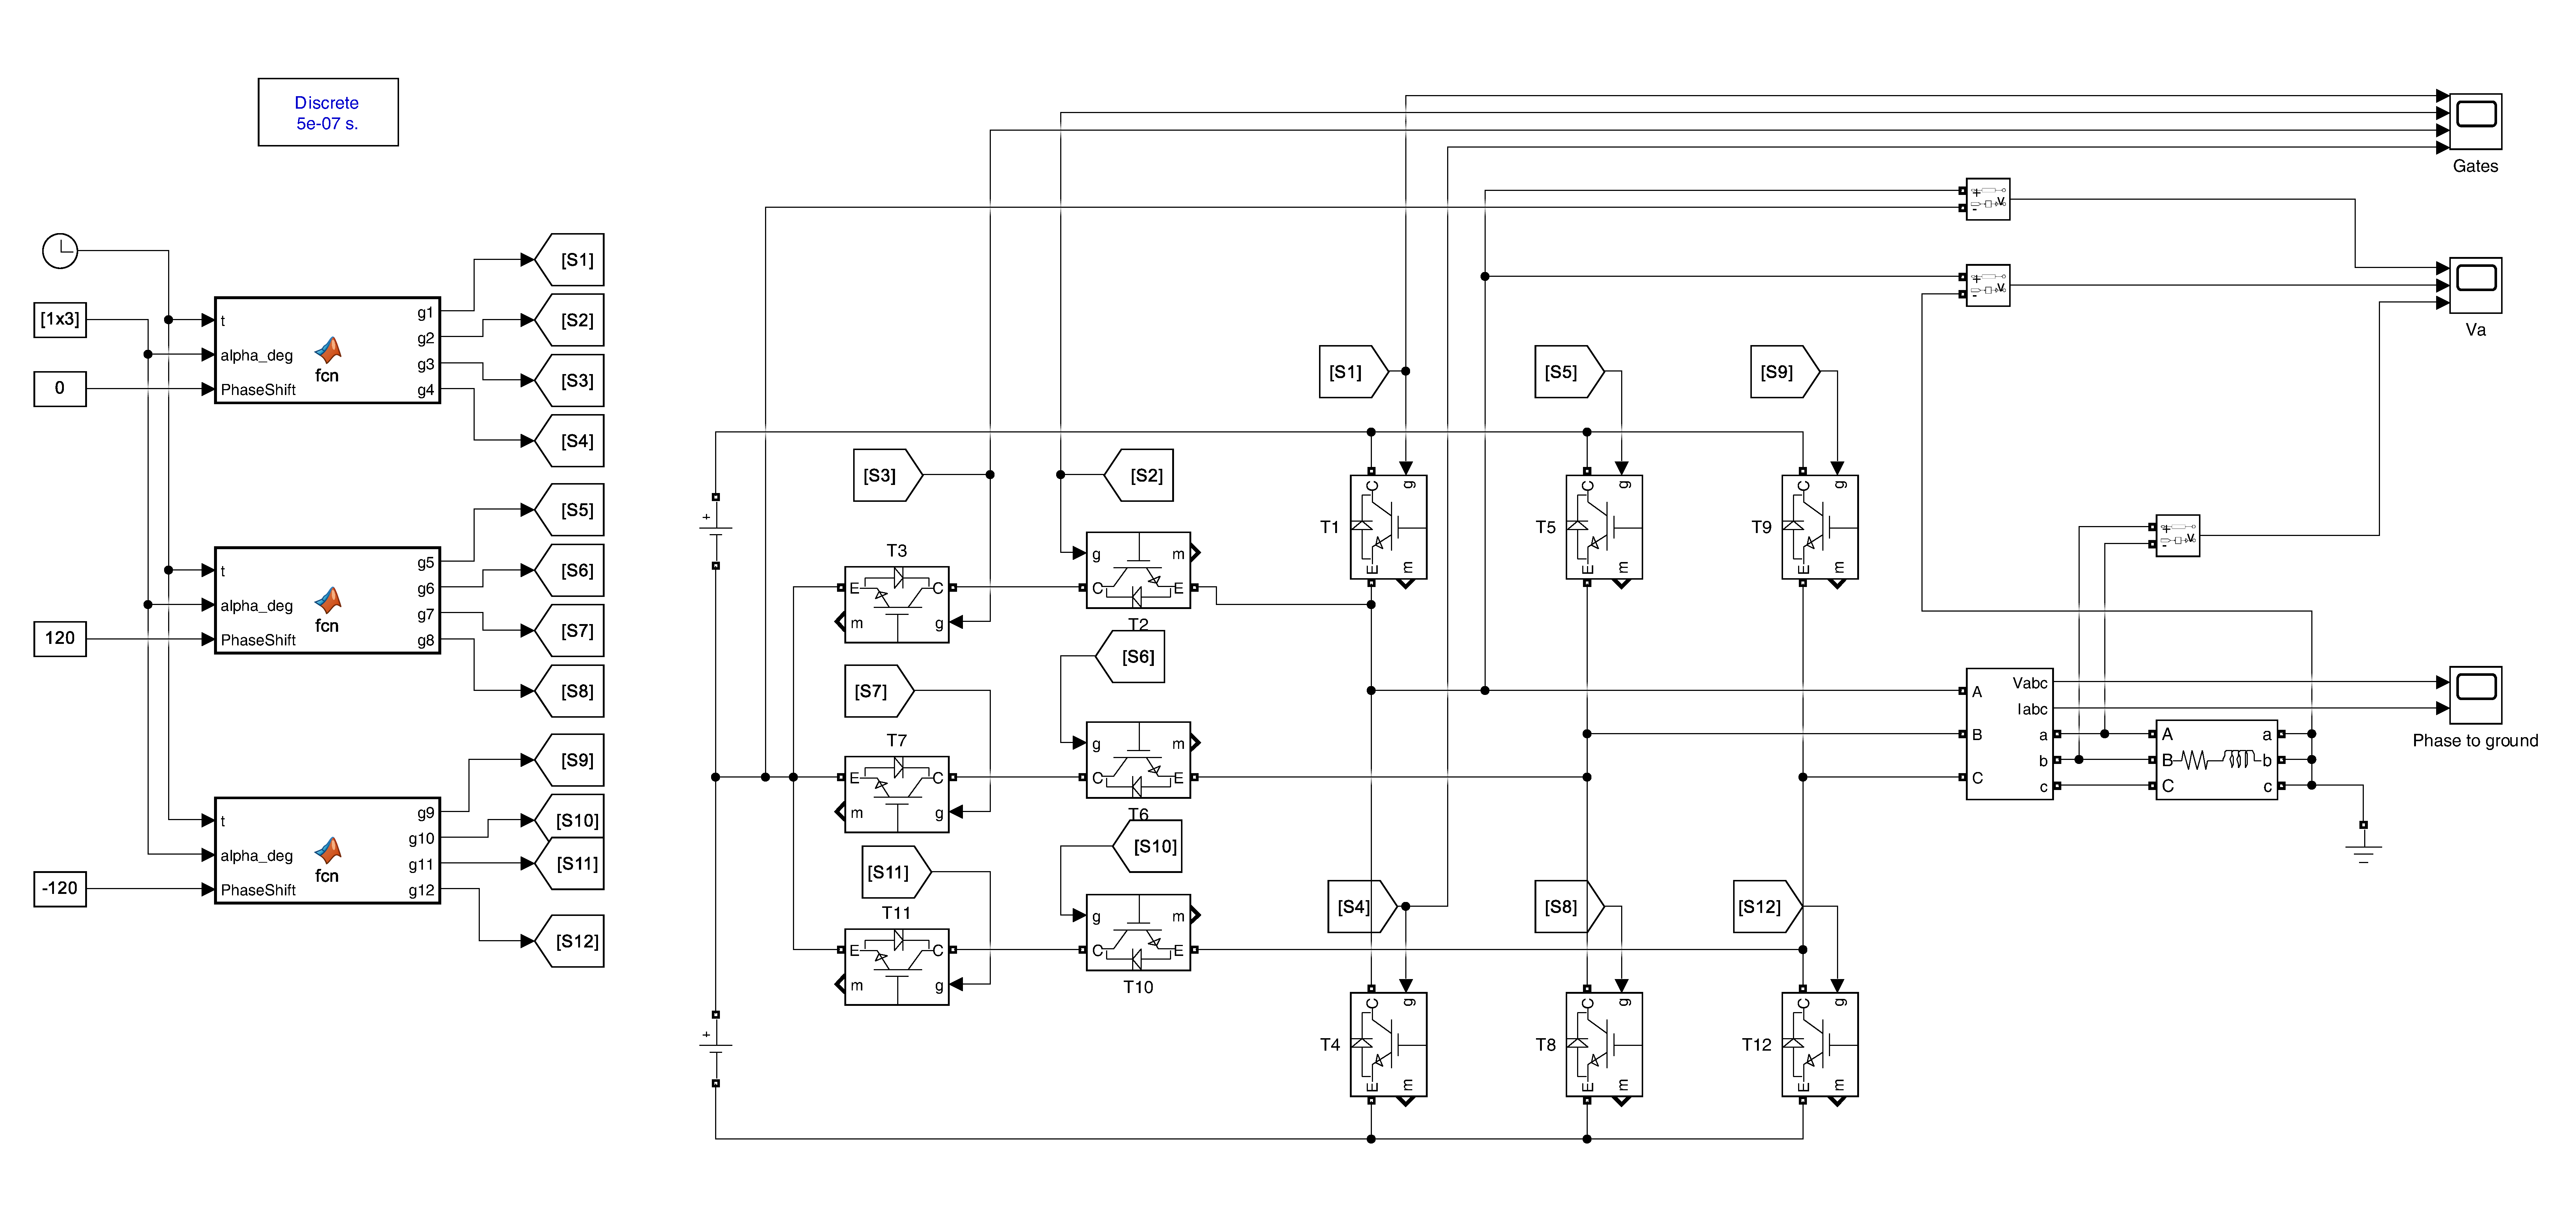
\includegraphics[width=\linewidth]{final_t_type_inverter.png}
		\caption{Simulink Schematic of the Three-Phase Three-Level T-Type Inverter}
	\end{figure}
	
	\subsection{Gate Pulse Generation Algorithm}
	The translation of calculated angles into real-time gate signals ($g_1, g_2, g_3, g_4$) is performed by a MATLAB Function block. The algorithm implements state-machine logic to manage transitions between positive, negative, and zero voltage levels.
	
	\begin{lstlisting}[caption=Gate Logic Implementation for T-Type Topology]
		function [g1, g2, g3, g4] = fcn(t, alpha_deg, PhaseShift)
		% 1. Frequency and Phase Synchronization
		Freq = 50; 
		w = 2*pi*Freq;
		theta = mod(w*t + PhaseShift*(pi/180), 2*pi);
		
		% 2. Angle Conversion
		a = alpha_deg * (pi/180);
		a1 = a(1); a2 = a(2); a3 = a(3);
		
		% 3. State Determination
		State = 0; 
		
		% Logic for Positive Half-Cycle
		if (theta < pi) 
		if (theta >= a1 && theta < a2) || ...
		(theta >= a3 && theta < (pi - a3)) || ...
		(theta >= (pi - a2) && theta < (pi - a1))
		State = 1;
		end
		else 
		% Logic for Negative Half-Cycle
		theta_rel = theta - pi;
		if (theta_rel >= a1 && theta_rel < a2) || ...
		(theta_rel >= a3 && theta_rel < (pi - a3)) || ...
		(theta_rel >= (pi - a2) && theta_rel < (pi - a1))
		State = -1;
		end
		end
		
		% 4. Signal Assignment (Optimized Neutral Path Control)
		g1 = 0; g2 = 0; g3 = 0; g4 = 0;
		
		switch State
		case 1      % Positive State (+Vdc/2)
		g1 = 1; % T1 Active
		case -1     % Negative State (-Vdc/2)
		g4 = 1; % T4 Active
		otherwise   % Zero State (0V) - Critical Fix
		g2 = 1; % Engage Neutral Path High-Side
		g3 = 1; % Engage Neutral Path Low-Side
		end
		end
	\end{lstlisting}
	
	\section{Development of Automated Analysis Tool}
	To facilitate rapid design iteration and performance validation, a custom MATLAB-based Graphical User Interface (GUI) application, titled the \textit{SHE Inverter Analysis Tool}, was developed. This tool integrates the mathematical solver with a time-domain simulation engine.
	
	\subsection{Functional Architecture}
	The tool is structured into three primary functional modules:
	\begin{enumerate}
		\item \textbf{Configuration Interface:} Allows the user to define system parameters such as DC link voltage, target fundamental voltage, and load impedance. It also accepts initial guesses for the Newton-Raphson solver to ensure convergence.
		\item \textbf{Computational Engine:}
		\begin{itemize}
			\item \textbf{SHE Solver:} Utilizes the \texttt{fsolve} function to numerically solve the non-linear transcendental equations for $\alpha_1, \alpha_2, \alpha_3$.
			\item \textbf{Waveform Synthesis:} Reconstructs the theoretical voltage and current waveforms based on the computed angles and load characteristics.
			\item \textbf{FFT Processor:} Performs Fast Fourier Transform analysis to compute harmonic magnitudes and Total Harmonic Distortion (THD).
		\end{itemize}
		\item \textbf{Visualization Dashboard:} A multi-tabbed interface that displays time-domain voltage waveforms ($V_{ao}, V_{an}, V_{ab}$), frequency-domain spectra, and instantaneous power flow.
	\end{enumerate}
	\newpage
	
	\section{Gate Drive Logic \& Neutral Point Control}
	A critical design requirement for the T-Type topology is the explicit control of the neutral point switches (T2 and T3) during the zero-voltage state. Unlike 2-level inverters, the output must be actively clamped to the neutral point to prevent floating potentials.
	
	\subsection{Logic Optimization \& Correction}
	Figure \ref{fig:gate_compare} illustrates the distinction between the initial implementation and the corrected logic.
	
	\begin{figure}[H]
		\centering
		% Stacked vertically with constrained height
		\begin{subfigure}[b]{1.0\linewidth}
			\centering
			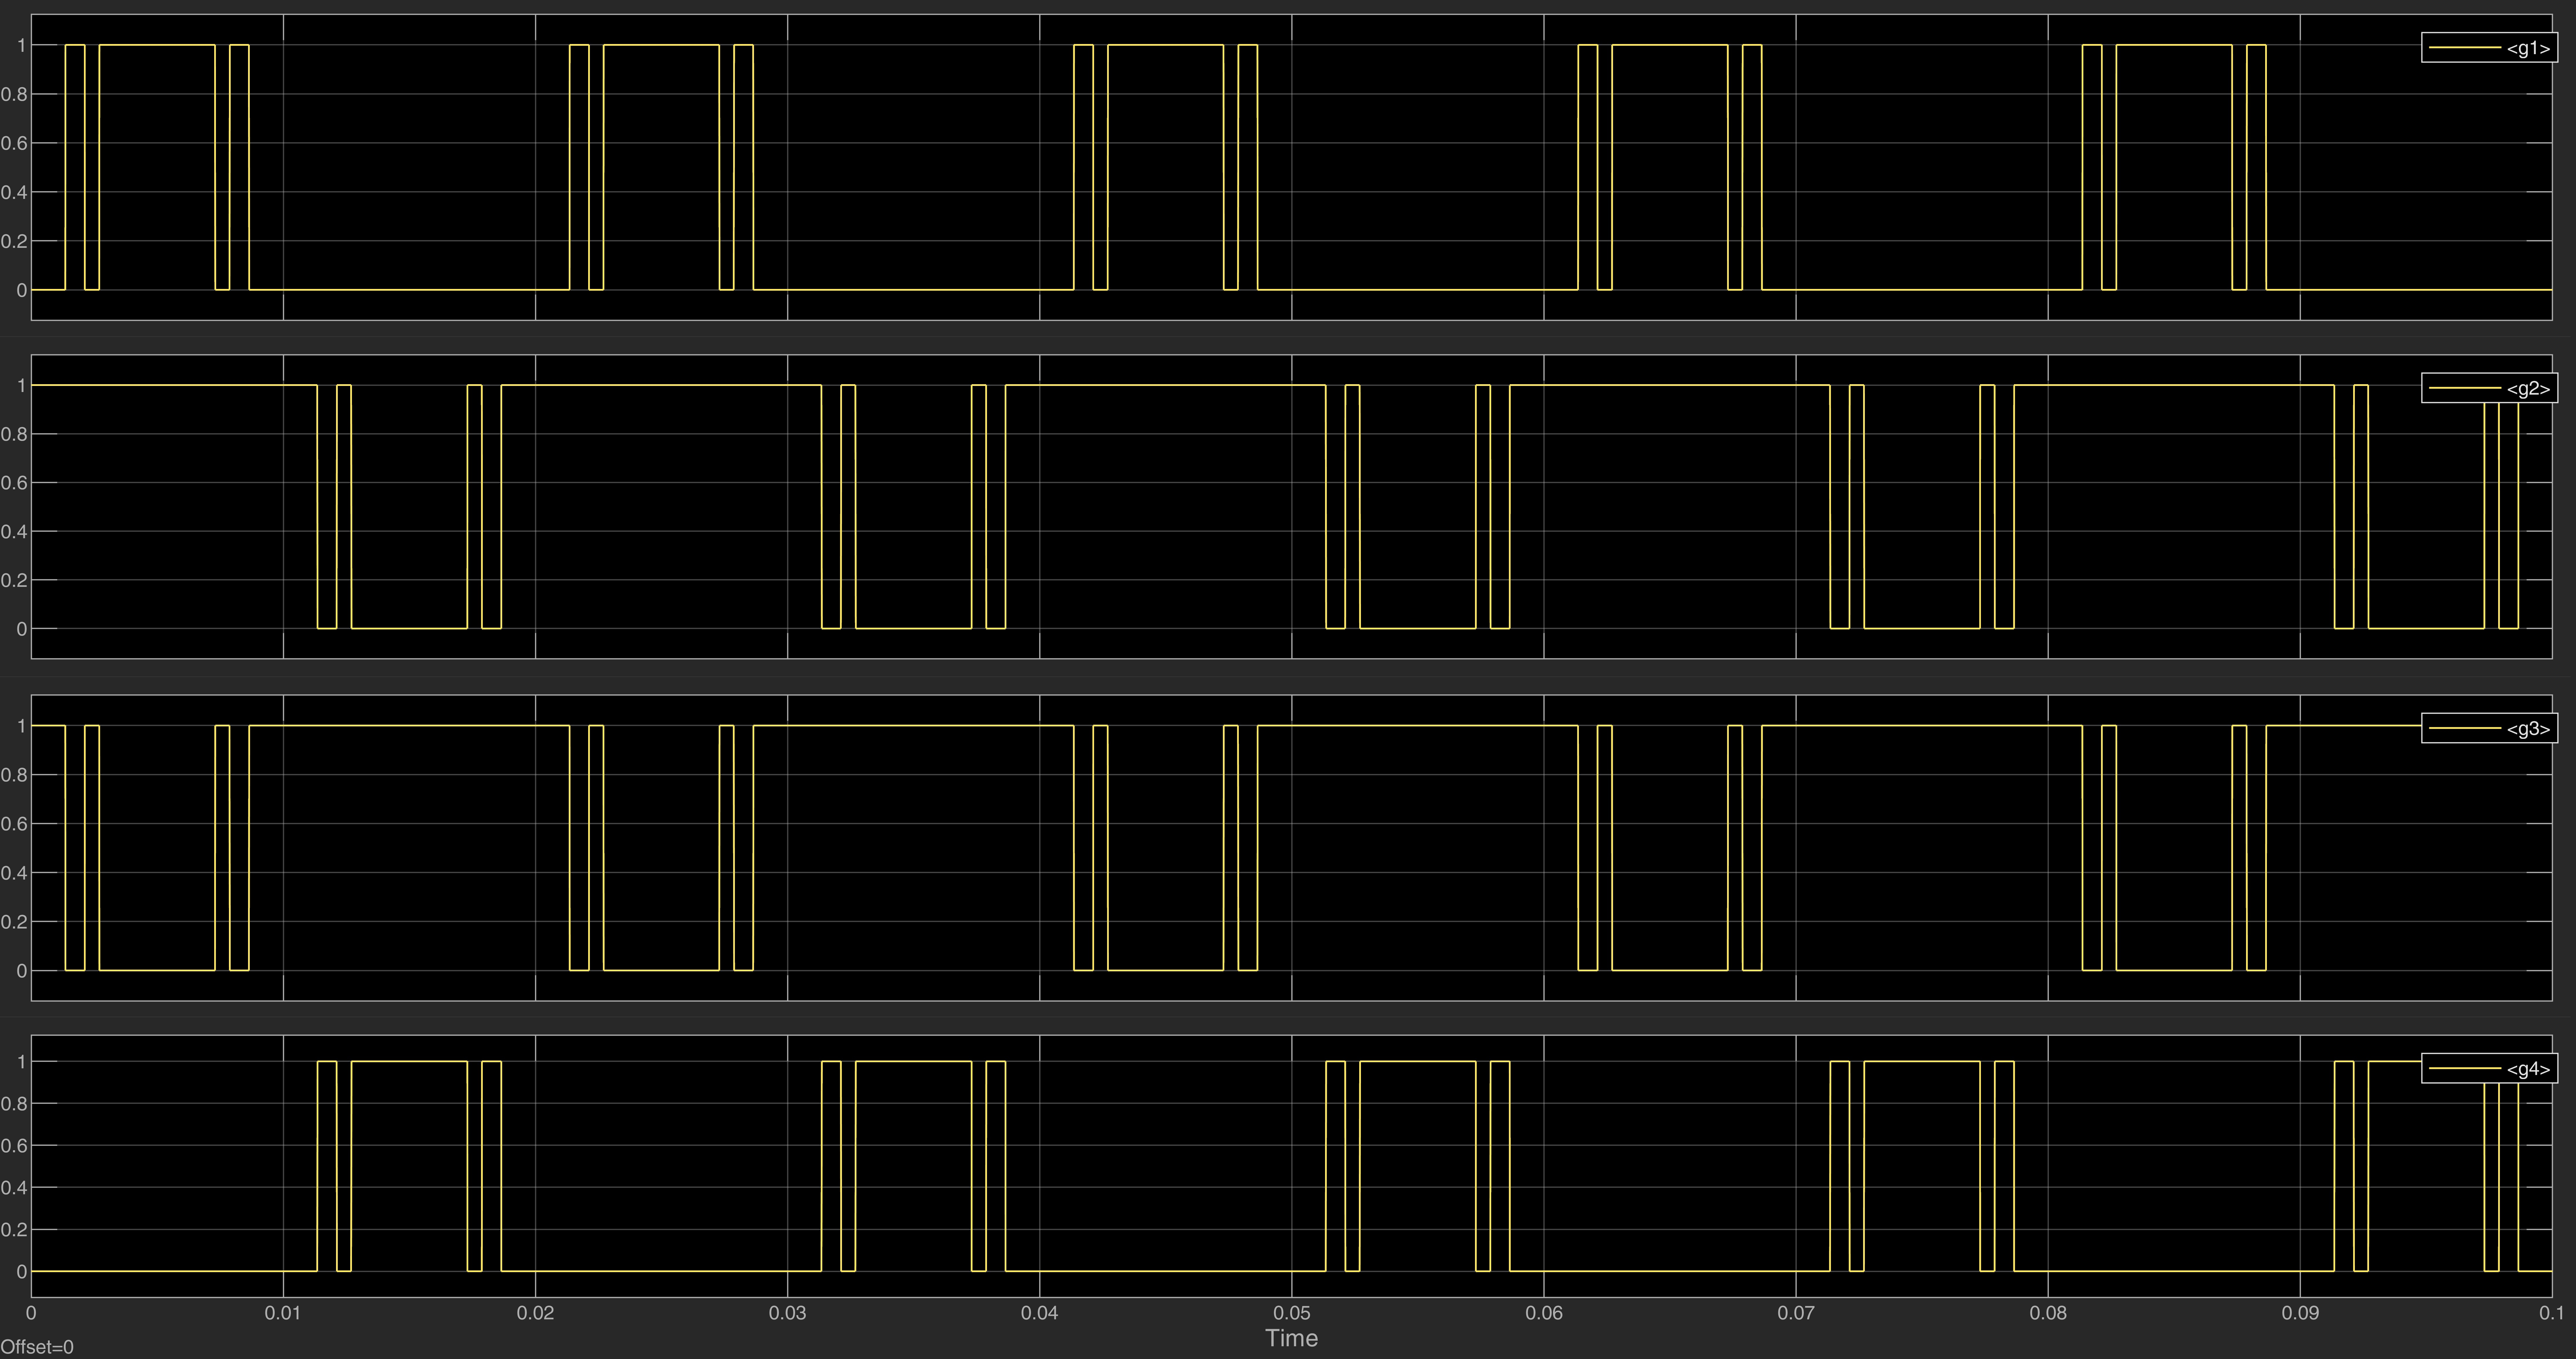
\includegraphics[width=\linewidth, height=6cm, keepaspectratio]{Gates_Old.jpg}
			\caption{\textbf{Initial Logic:} Note the undefined states and lack of active clamping.}
		\end{subfigure}
		
		\vspace{0.3cm} % Small vertical space
		
		\begin{subfigure}[b]{1.0\linewidth}
			\centering
			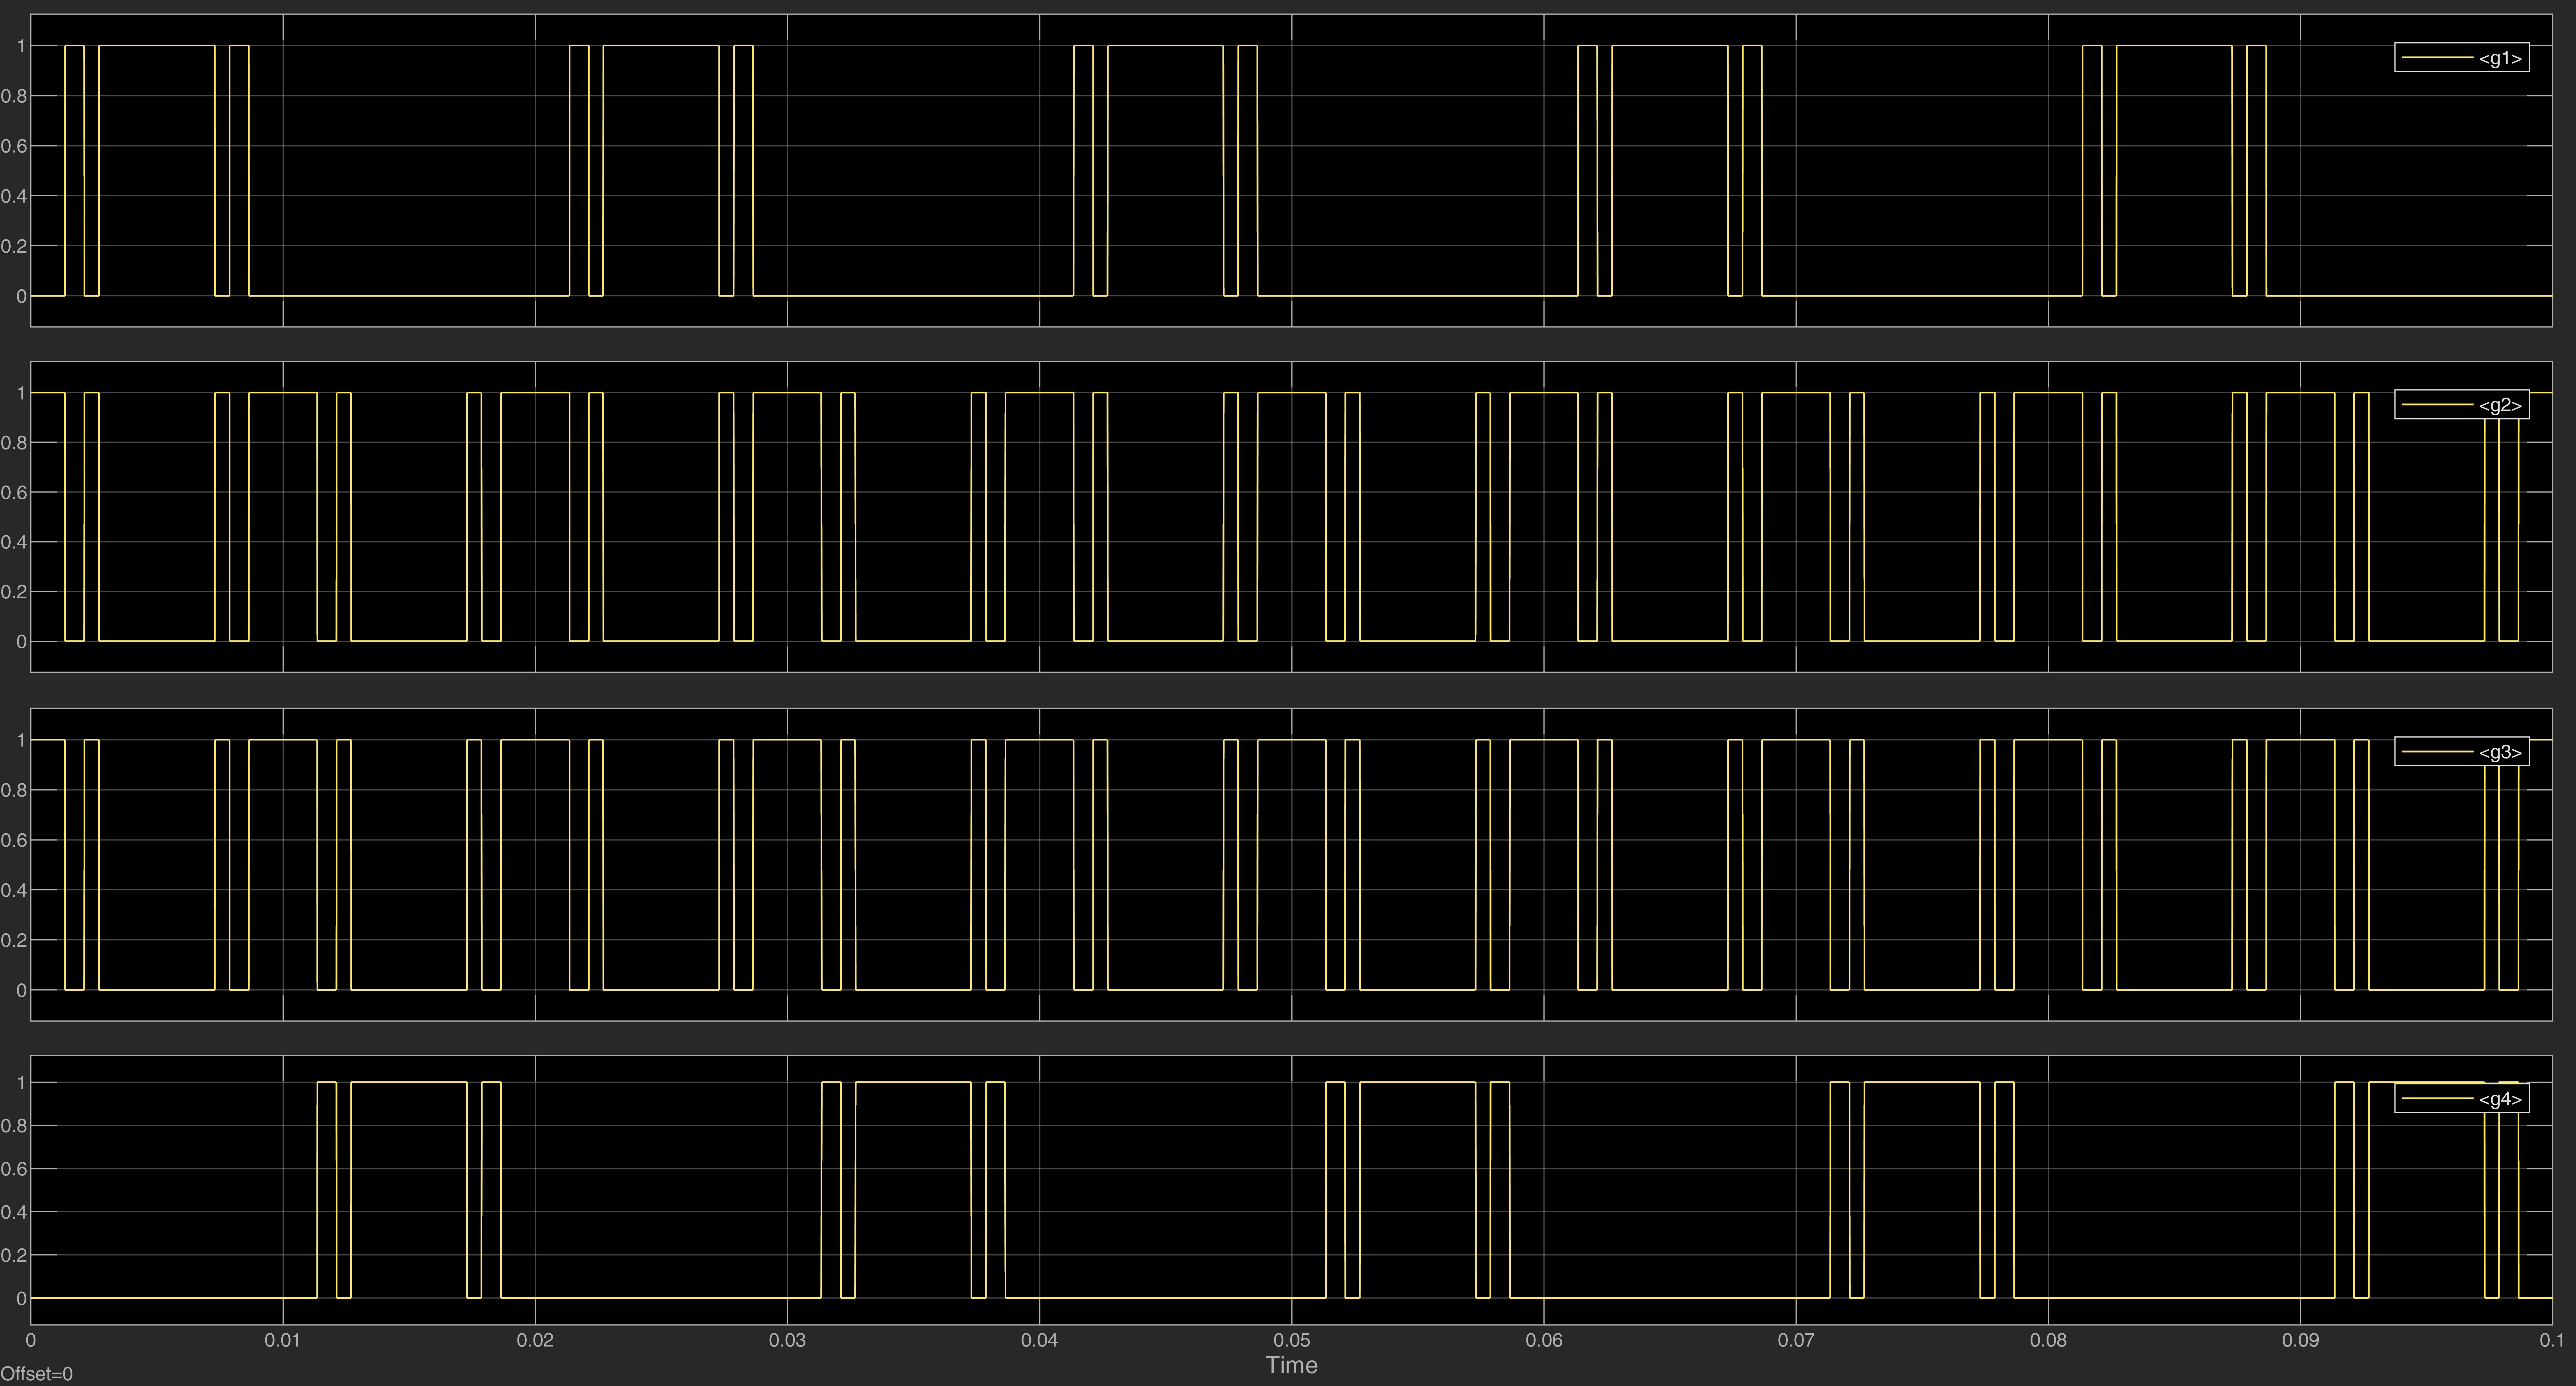
\includegraphics[width=\linewidth, height=6cm, keepaspectratio]{Gates_New.jpg}
			\caption{\textbf{Optimized Logic:} Distinct transitions with T2/T3 actively engaged during zero states.}
		\end{subfigure}
		\caption{Comparative Analysis of Gate Drive Signals}
		\label{fig:gate_compare}
	\end{figure}
	
	\textbf{Technical Significance:}
	The optimized logic ensures that \textbf{both T2 and T3 are energized} whenever the output voltage is commanded to zero. This establishes a bidirectional current path to the neutral point ($O$). Without this mechanism, the output voltage would be dictated by parasitic load currents flowing through body diodes, resulting in severe waveform distortion and increased THD. The corrected signals demonstrate precise alignment with the theoretical SHE switching instances.
	
	\section{Voltage Waveform Analysis}
	
	\subsection{Pole Voltage Characteristics ($V_{ao}$)}
	The pole voltage represents the potential difference between phase A and the DC link midpoint.
	
	\begin{figure}[H]
		\centering
		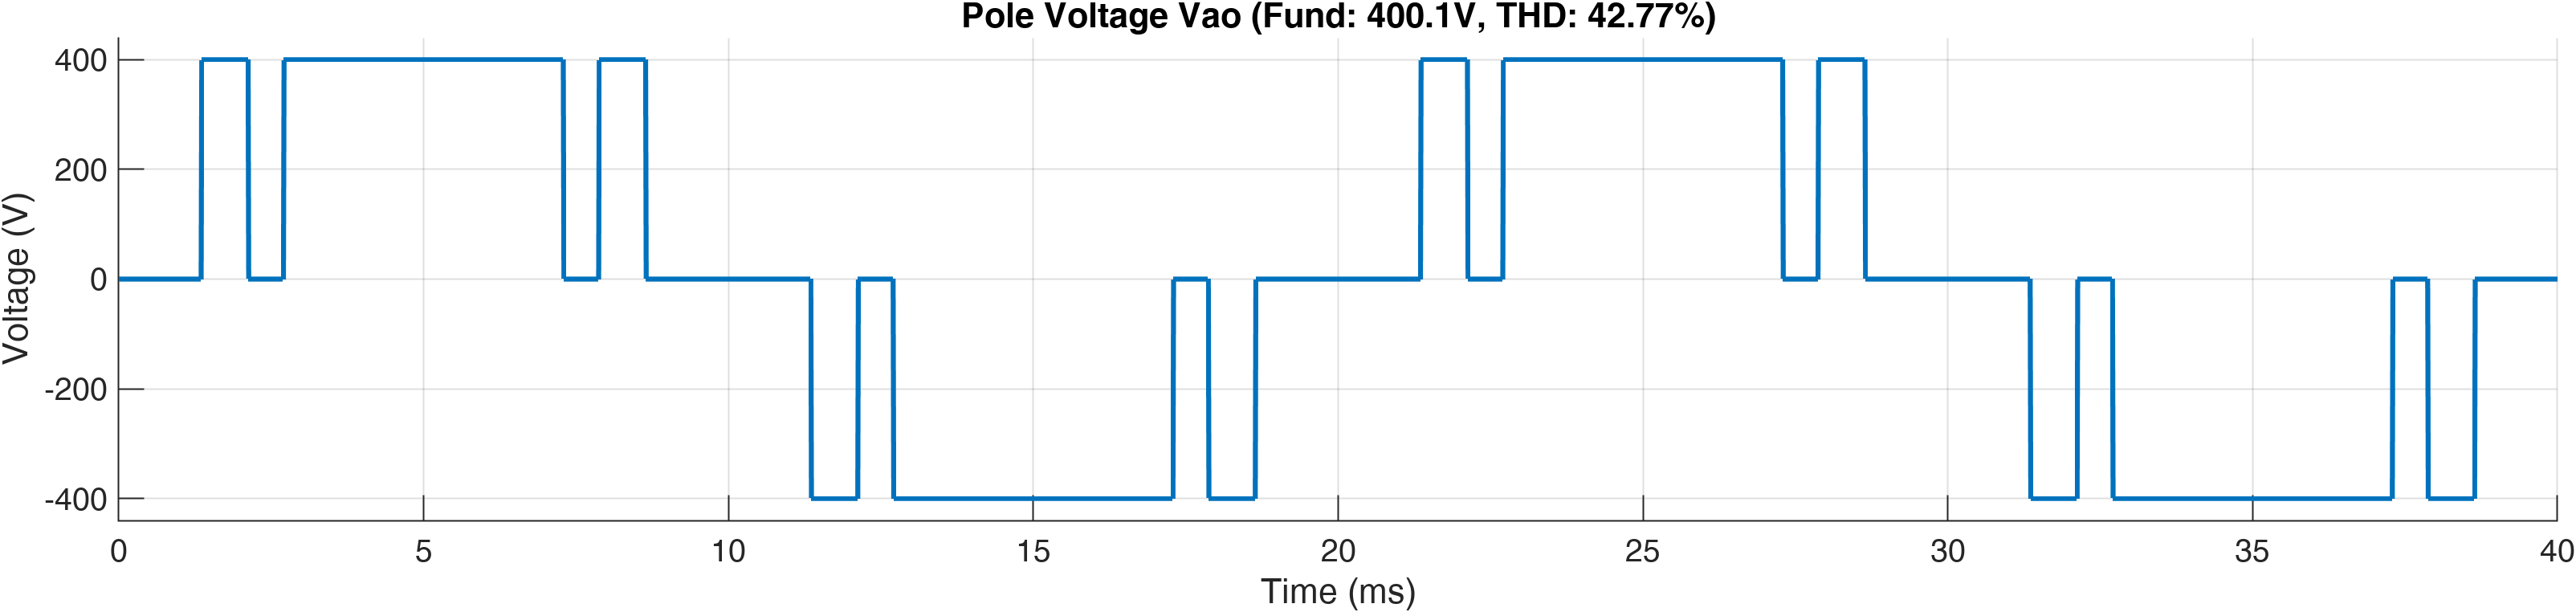
\includegraphics[width=\linewidth]{1_Pole_Voltage_Vao.png}
		\caption{Pole Voltage $V_{ao}$ Waveform}
	\end{figure}
	
	\textbf{Waveform Characteristics:}
	The signal exhibits a strict three-level structure switching between $+400\text{V}$, $0\text{V}$, and $-400\text{V}$. The pulse widths correspond exactly to the calculated SHE angles, verifying the correct implementation of the modulation strategy.
	
	\subsection{Phase and Line Voltage Synthesis}
	The phase voltage relative to the load neutral ($V_{an}$) and the line-to-line voltage ($V_{ab}$) are derived from the pole voltages.
	
	\begin{figure}[H]
		\centering
		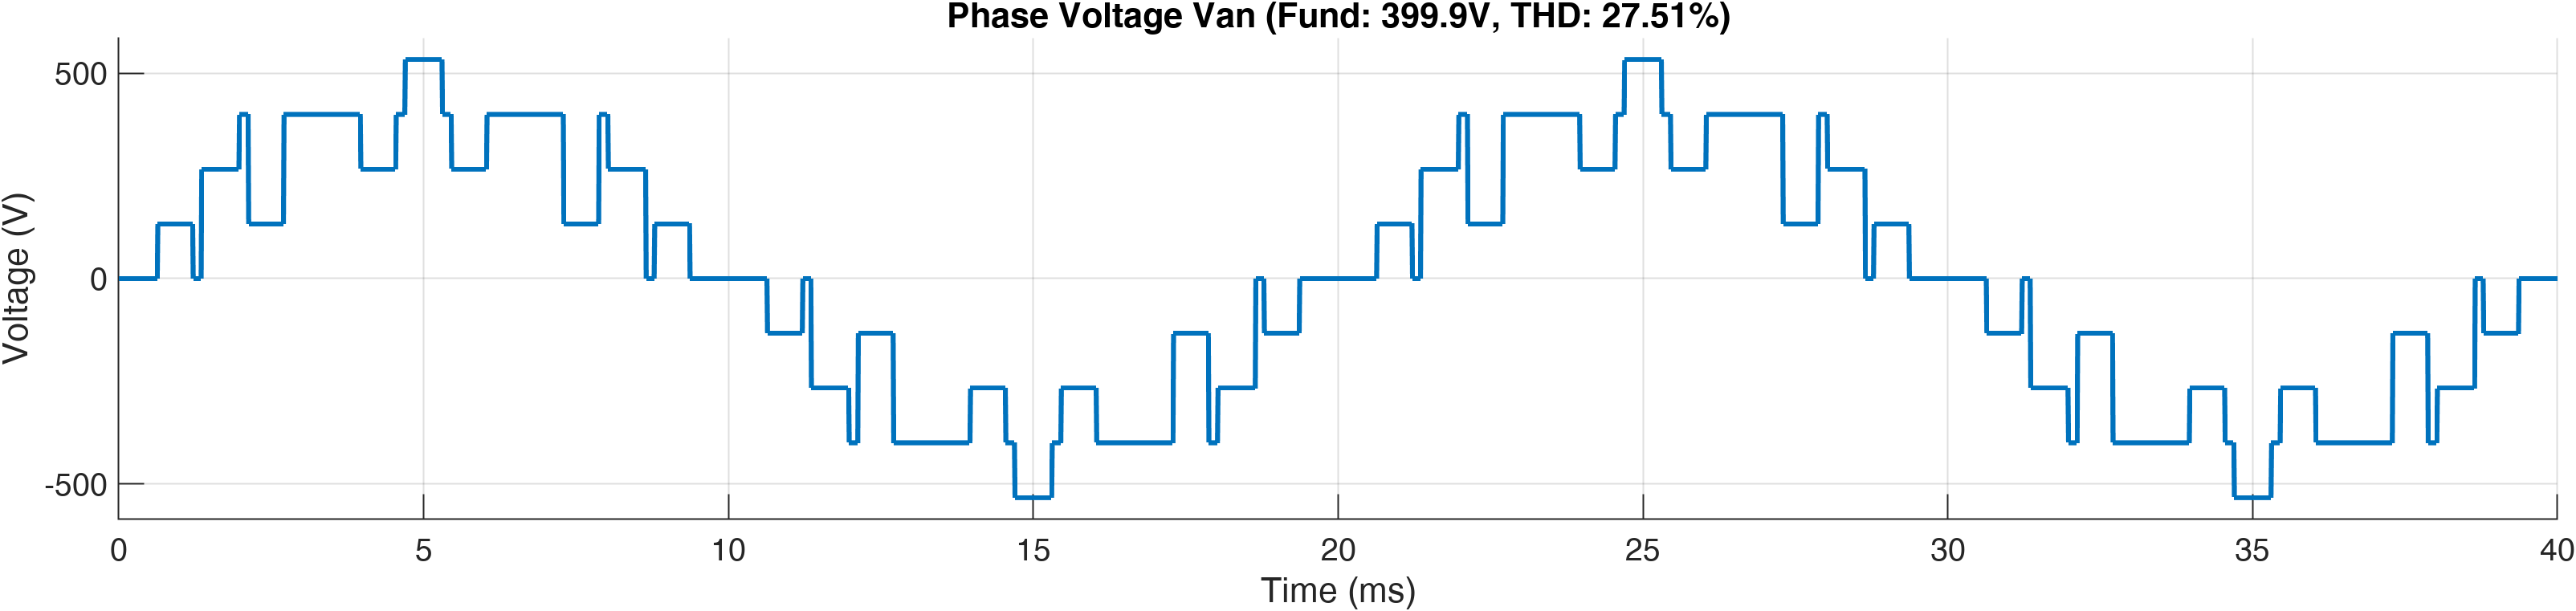
\includegraphics[width=\linewidth]{2_Phase_Voltage_Van.png}
		\caption{Phase Voltage $V_{an}$ Waveform}
	\end{figure}
	
	\textbf{Performance Analysis:}
	The phase voltage demonstrates a stepped approximation of a sine wave. The significant reduction in THD compared to the pole voltage is attributed to the cancellation of triplen harmonics inherent in the three-phase line-neutral configuration.
	
	\subsection{Line Voltage Characteristics ($V_{ab}$)}
	\begin{figure}[H]
		\centering
		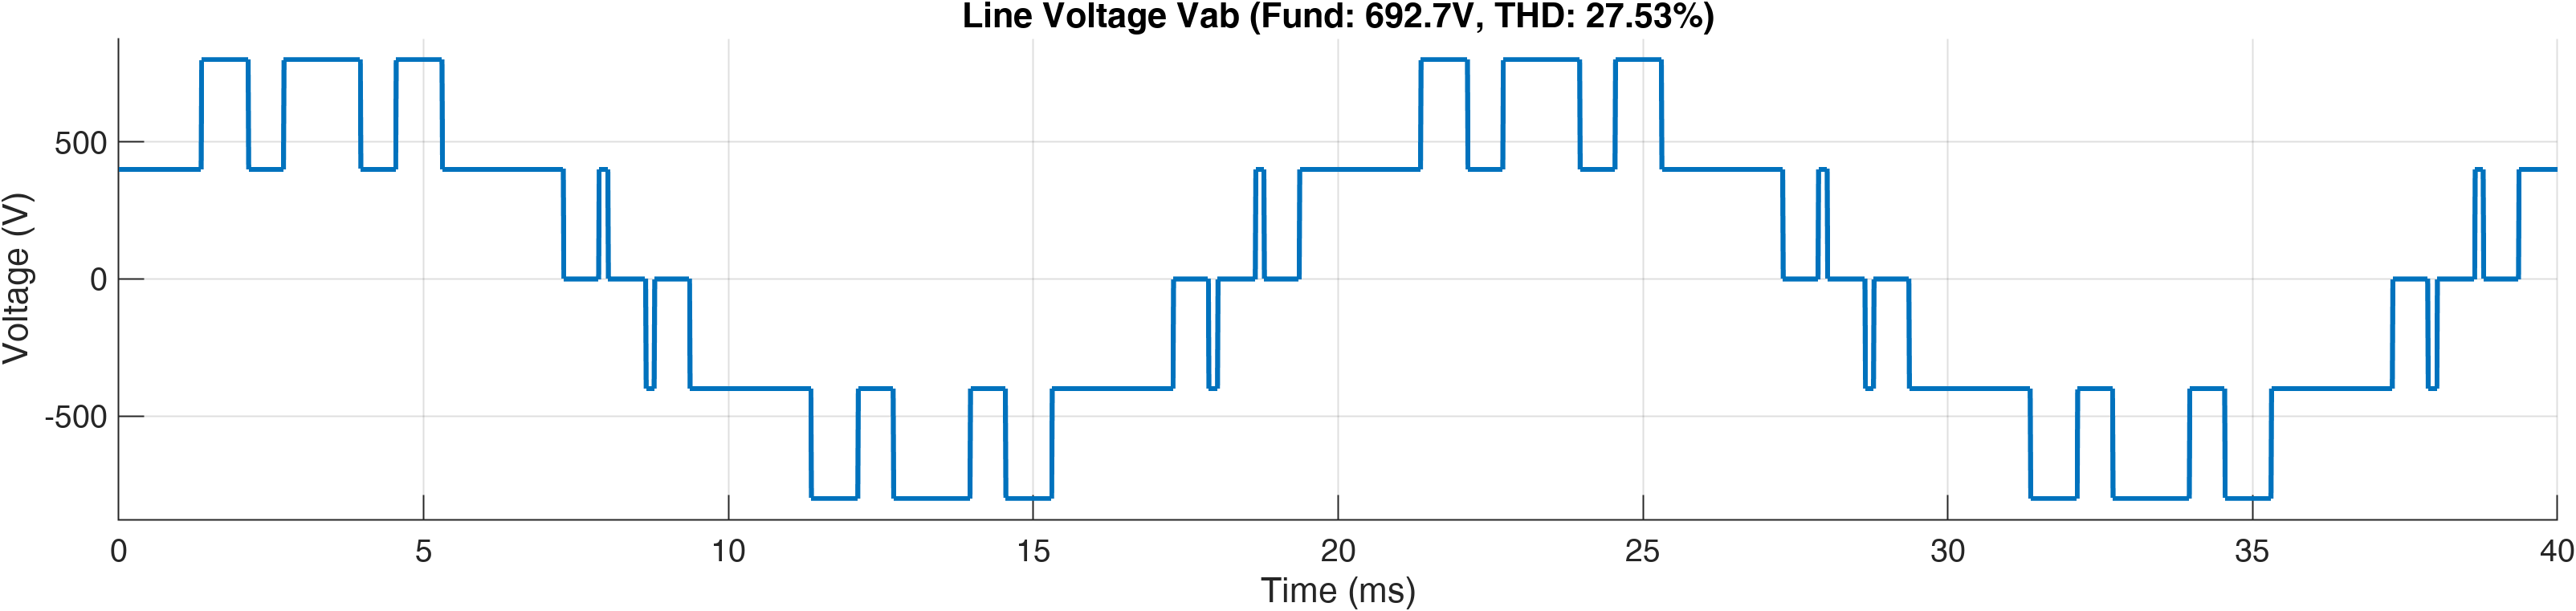
\includegraphics[width=\linewidth]{3_Line_Voltage_Vab.png}
		\caption{Line Voltage $V_{ab}$ Waveform}
	\end{figure}
	
	\textbf{Analysis:}
	The line voltage displays a 5-level staircase waveform ($+800, +400, 0, -400, -800$V). This increased number of levels significantly improves the harmonic spectrum compared to conventional topologies, reducing the filtering requirements.
	
	\section{Spectral Evaluation (FFT)}
	
	\subsection{Voltage Harmonic Distribution}
	Fast Fourier Transform (FFT) analysis was conducted to quantify the harmonic content and verify the elimination of targeted orders.
	
	\textbf{Pole Voltage Spectra:}
	\begin{figure}[H]
		\centering
		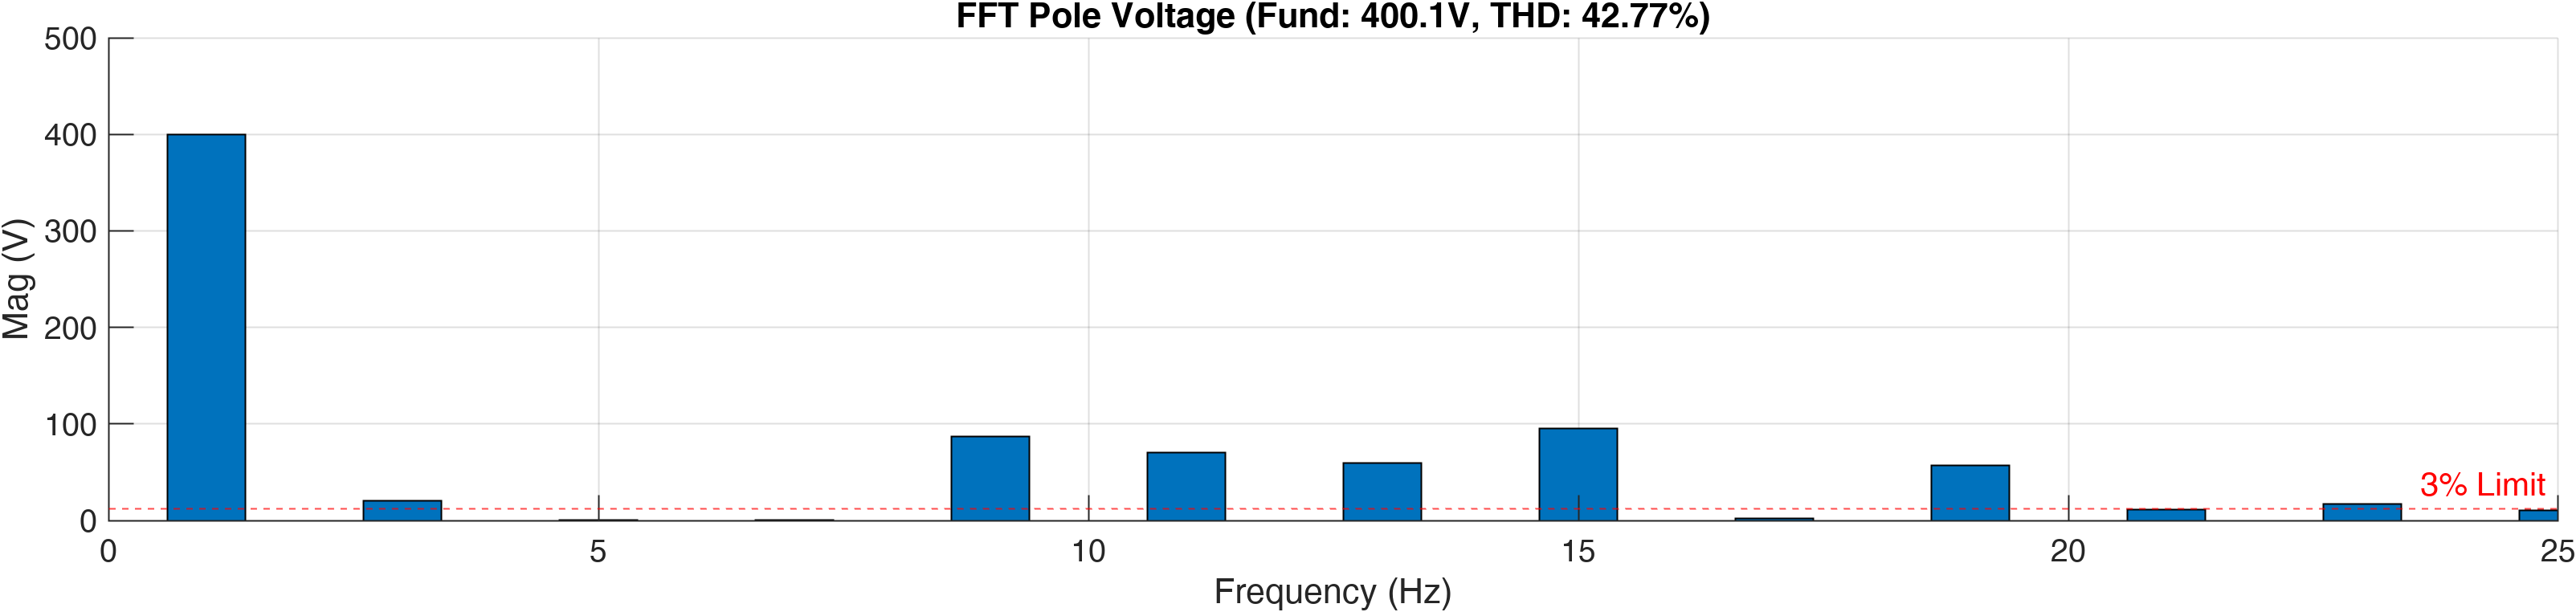
\includegraphics[width=\linewidth]{4_FFT_Pole_Voltage.png}
		\caption{FFT of Pole Voltage $V_{ao}$}
	\end{figure}
	
	\textbf{Quantitative Validation:}
	Table \ref{tab:harmonics} presents the specific magnitudes of the targeted harmonics, confirming their successful elimination.
	
	\begin{table}[H]
		\centering
		\caption{Harmonic Magnitude Analysis (Pole Voltage)}
		\label{tab:harmonics}
		\begin{tabular}{ccc}
			\toprule
			\textbf{Harmonic Order ($n$)} & \textbf{Frequency (Hz)} & \textbf{Magnitude (V)} \\
			\midrule
			Fundamental ($1^{st}$) & 50 & 400.1 \\
			$5^{th}$ & 250 & $\approx 0.0$ \\
			$7^{th}$ & 350 & $\approx 0.0$ \\
			$11^{th}$ & 550 & 48.3 \\
			\bottomrule
		\end{tabular}
	\end{table}
	
	\vspace{2cm}
	\textbf{Line Voltage Spectra:}
	\begin{figure}[H]
		\centering
		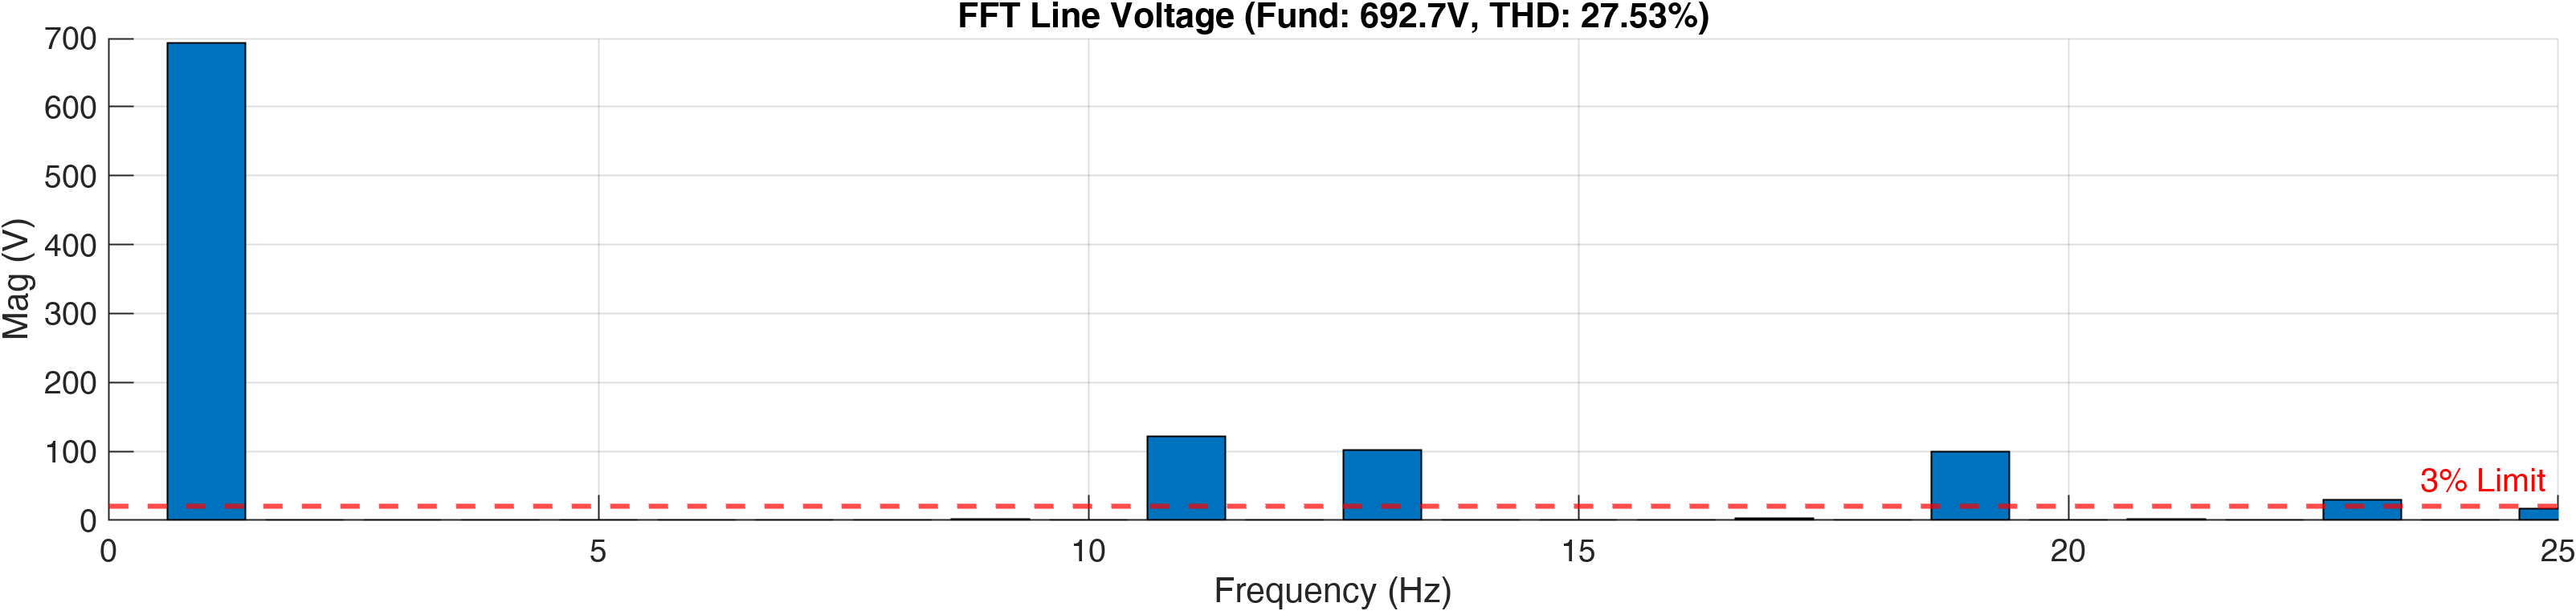
\includegraphics[width=\linewidth]{6_FFT_Line_Voltage.png}
		\caption{FFT of Line Voltage $V_{ab}$}
	\end{figure}
	
	\subsection{Current Harmonic Distortion}
	The inductive nature of the load acts as a low-pass filter, smoothing the current waveforms.
	
	\begin{figure}[H]
		\centering
		\begin{subfigure}[b]{0.32\textwidth}
			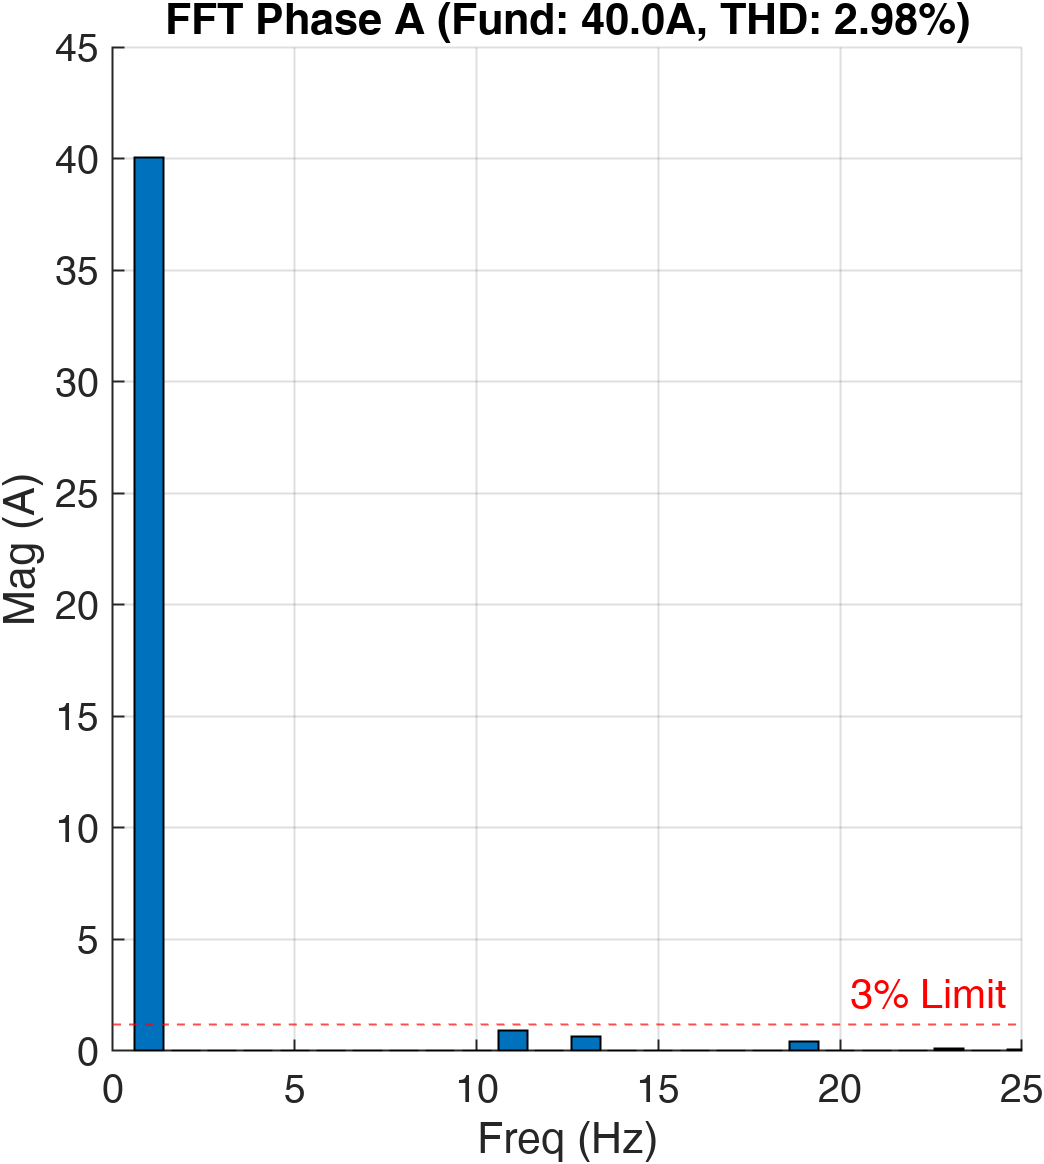
\includegraphics[width=\linewidth]{8_FFT_Current_PhaseA.png}
			\caption{Phase A (THD: 2.98\%)}
		\end{subfigure}
		\hfill
		\begin{subfigure}[b]{0.32\textwidth}
			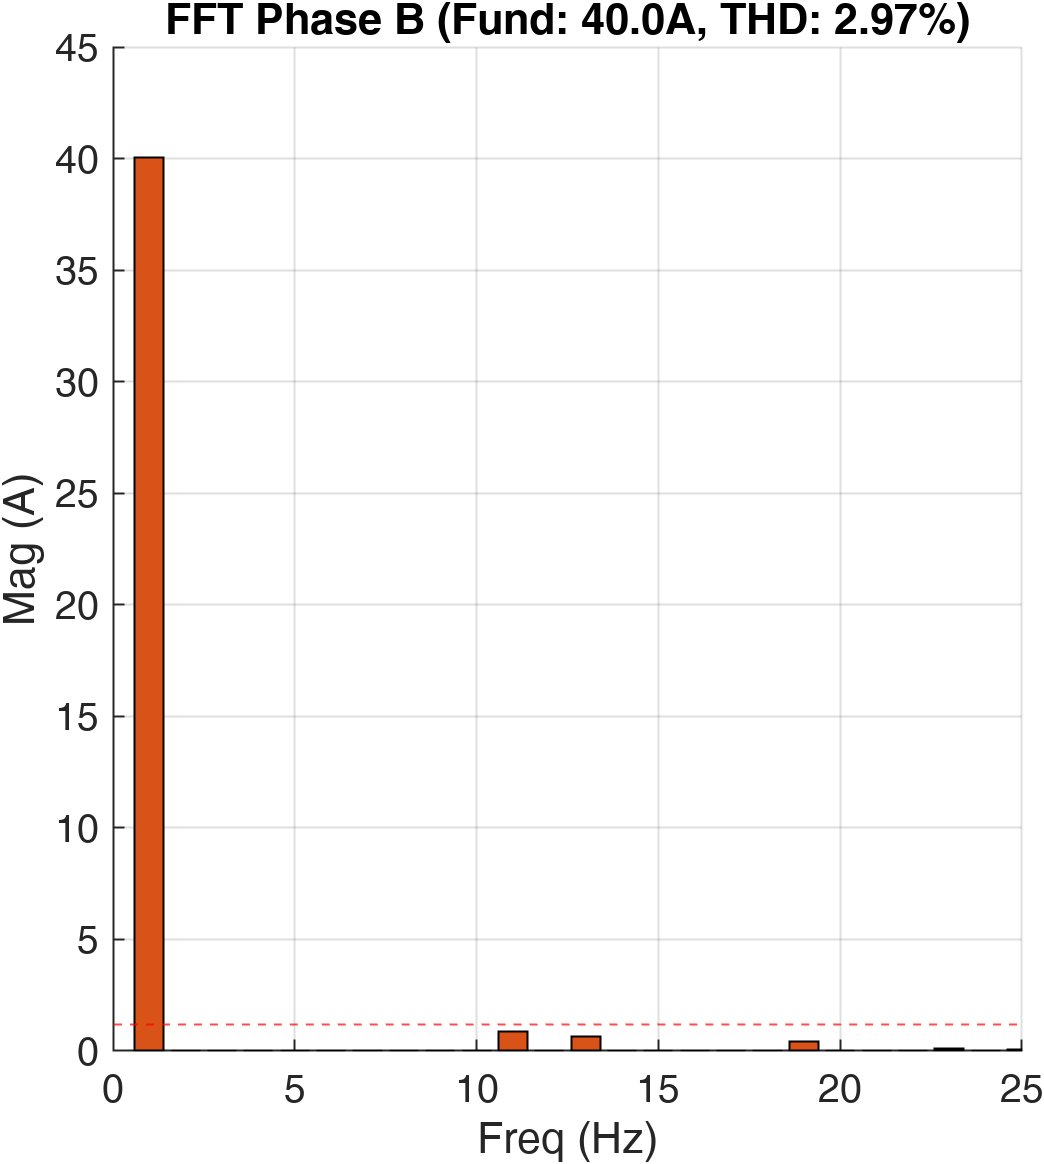
\includegraphics[width=\linewidth]{9_FFT_Current_PhaseB.png}
			\caption{Phase B (THD: 2.97\%)}
		\end{subfigure}
		\hfill
		\begin{subfigure}[b]{0.32\textwidth}
			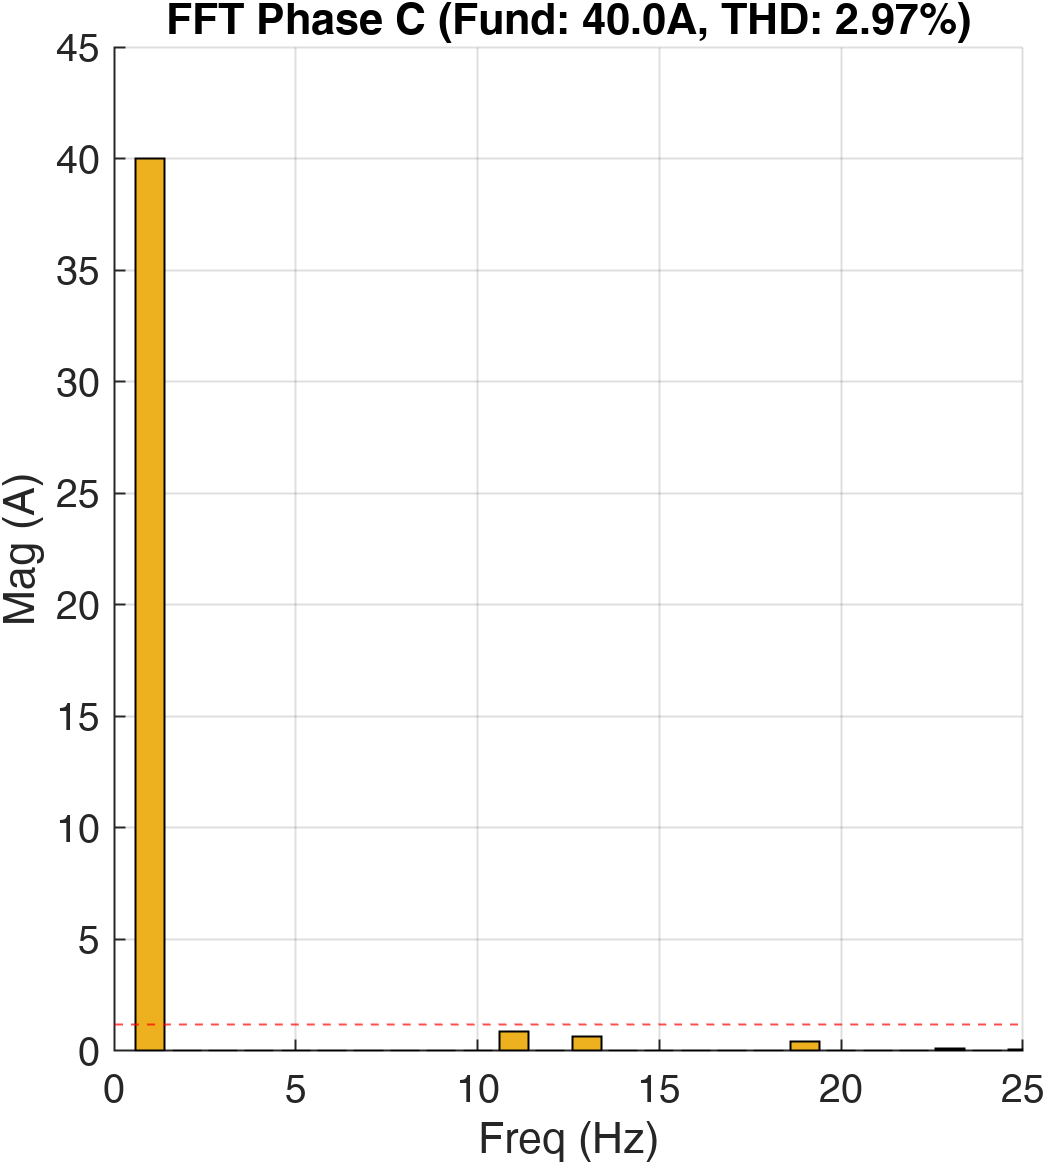
\includegraphics[width=\linewidth]{10_FFT_Current_PhaseC.png}
			\caption{Phase C (THD: 2.97\%)}
		\end{subfigure}
		\caption{FFT Analysis of Three-Phase Load Currents}
	\end{figure}
	
	\textbf{Performance Evaluation:}
	The measured Total Harmonic Distortion (THD) is approximately \textbf{2.98\%} across all phases. This value is well within international standards (typically $<5\%$), validating the effectiveness of the combined T-Type topology and SHE control strategy.
	
	\newpage
	\section{Current Waveform Characteristics}
	The time-domain current waveforms illustrate the balanced nature of the system. The currents are highly sinusoidal with minimal switching ripple. The peak amplitude aligns with the theoretical value derived from the load impedance: $I_{peak} \approx 40\text{A}$. This smooth profile indicates that the inductive load effectively filters out the higher-order harmonics generated by the switching process, leaving a clean fundamental component.
	
	\begin{figure}[H]
		\centering
		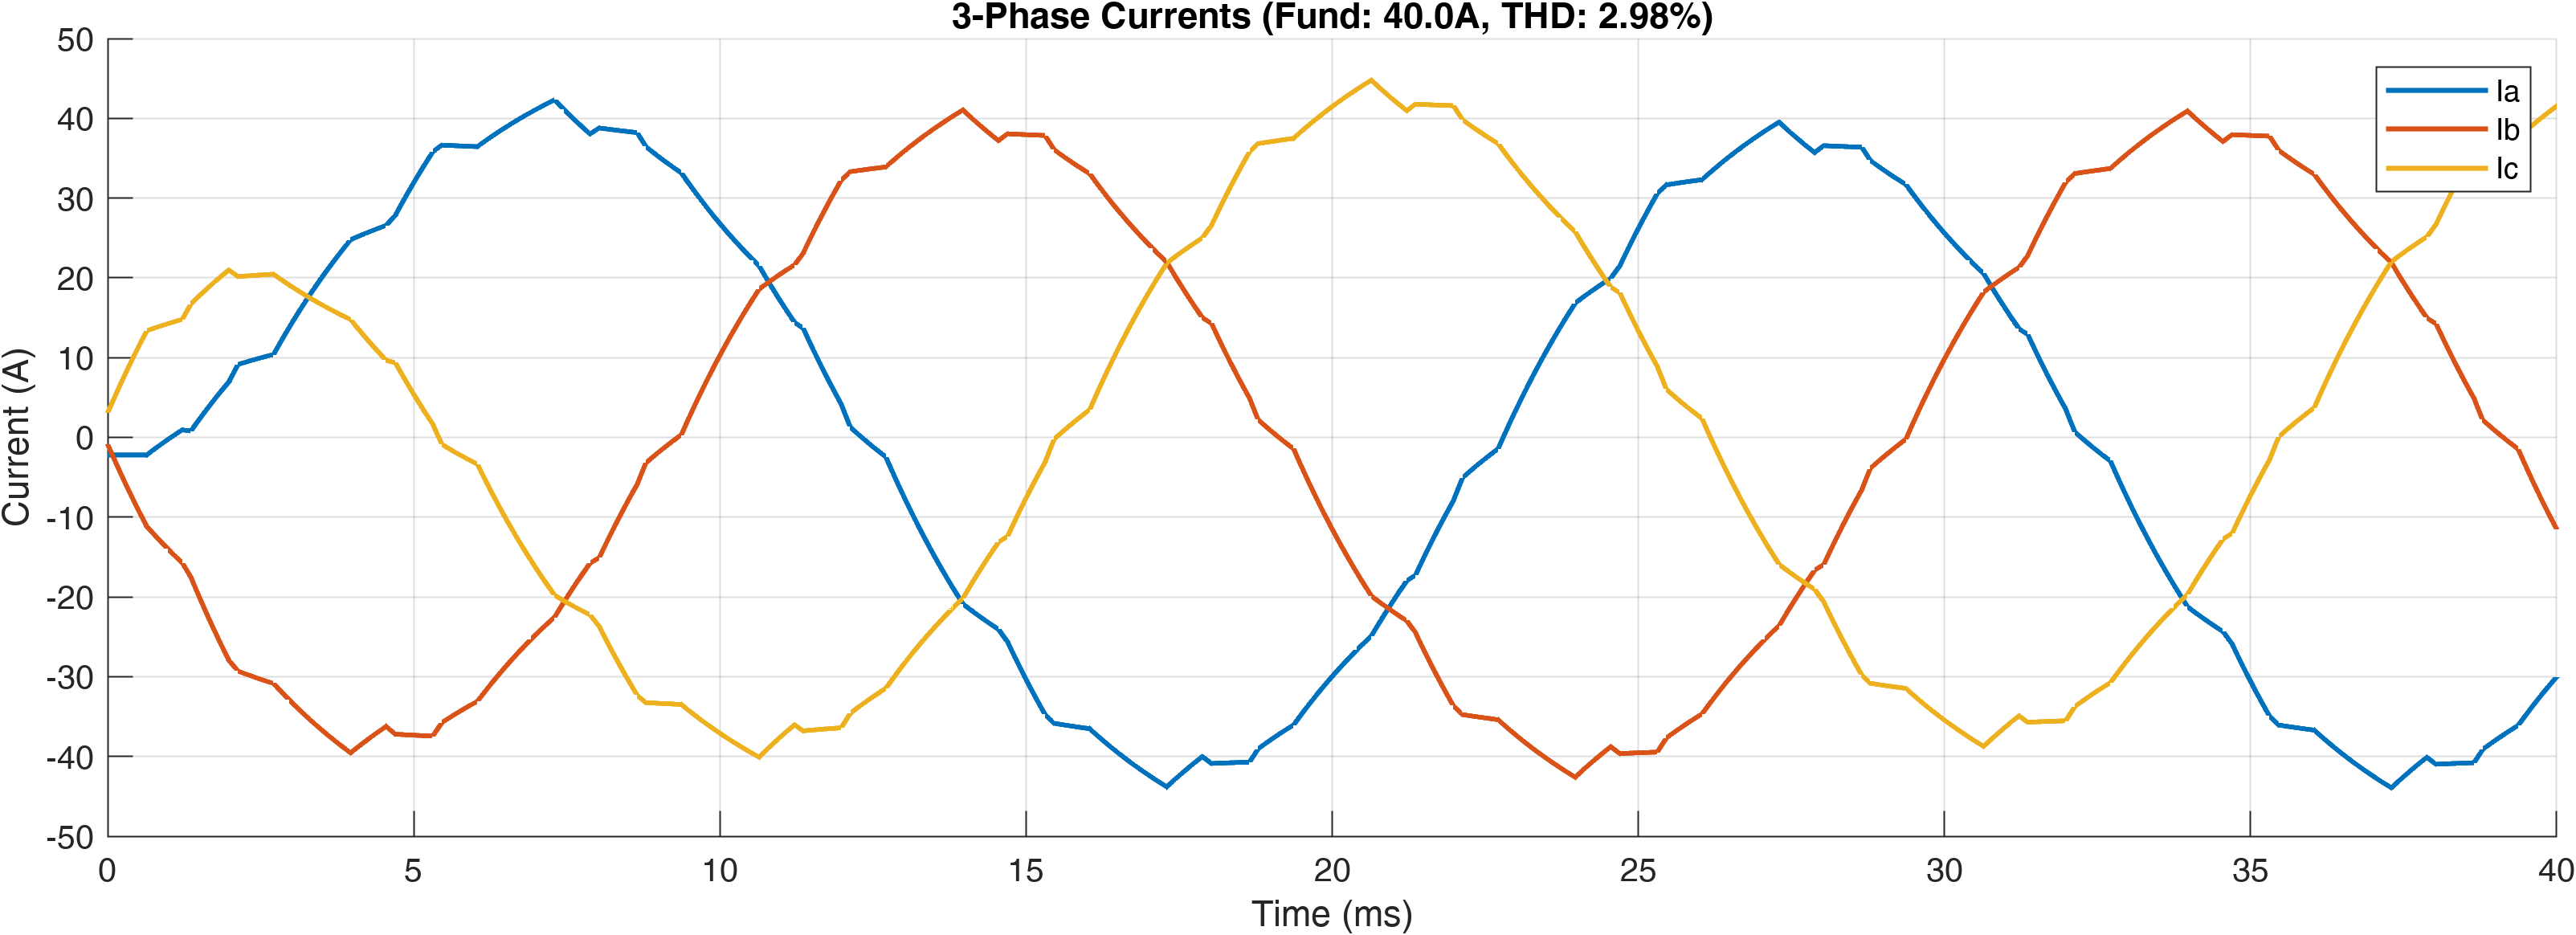
\includegraphics[width=\linewidth]{7_Current_Waveforms_Time.png}
		\caption{Three-Phase Load Currents ($I_a, I_b, I_c$)}
	\end{figure}
	
	\newpage
	
	\section{Power Flow Analysis}
	\begin{table}[H]
		\centering
		\caption{Power Performance Metrics}
		\begin{tabular}{lc}
			\toprule
			\textbf{Metric} & \textbf{Value} \\
			\midrule
			Active Power ($P$) & $16.98\text{kW}$ \\
			Reactive Power ($Q$) & $18.81\text{kVAR}$ \\
			Apparent Power ($S$) & $25.34\text{kVA}$ \\
			Power Factor ($PF$) & $0.67$ \\
			Estimated Efficiency & $97.7\%$ \\
			\bottomrule
		\end{tabular}
	\end{table}
	
	\begin{figure}[H]
		\centering
		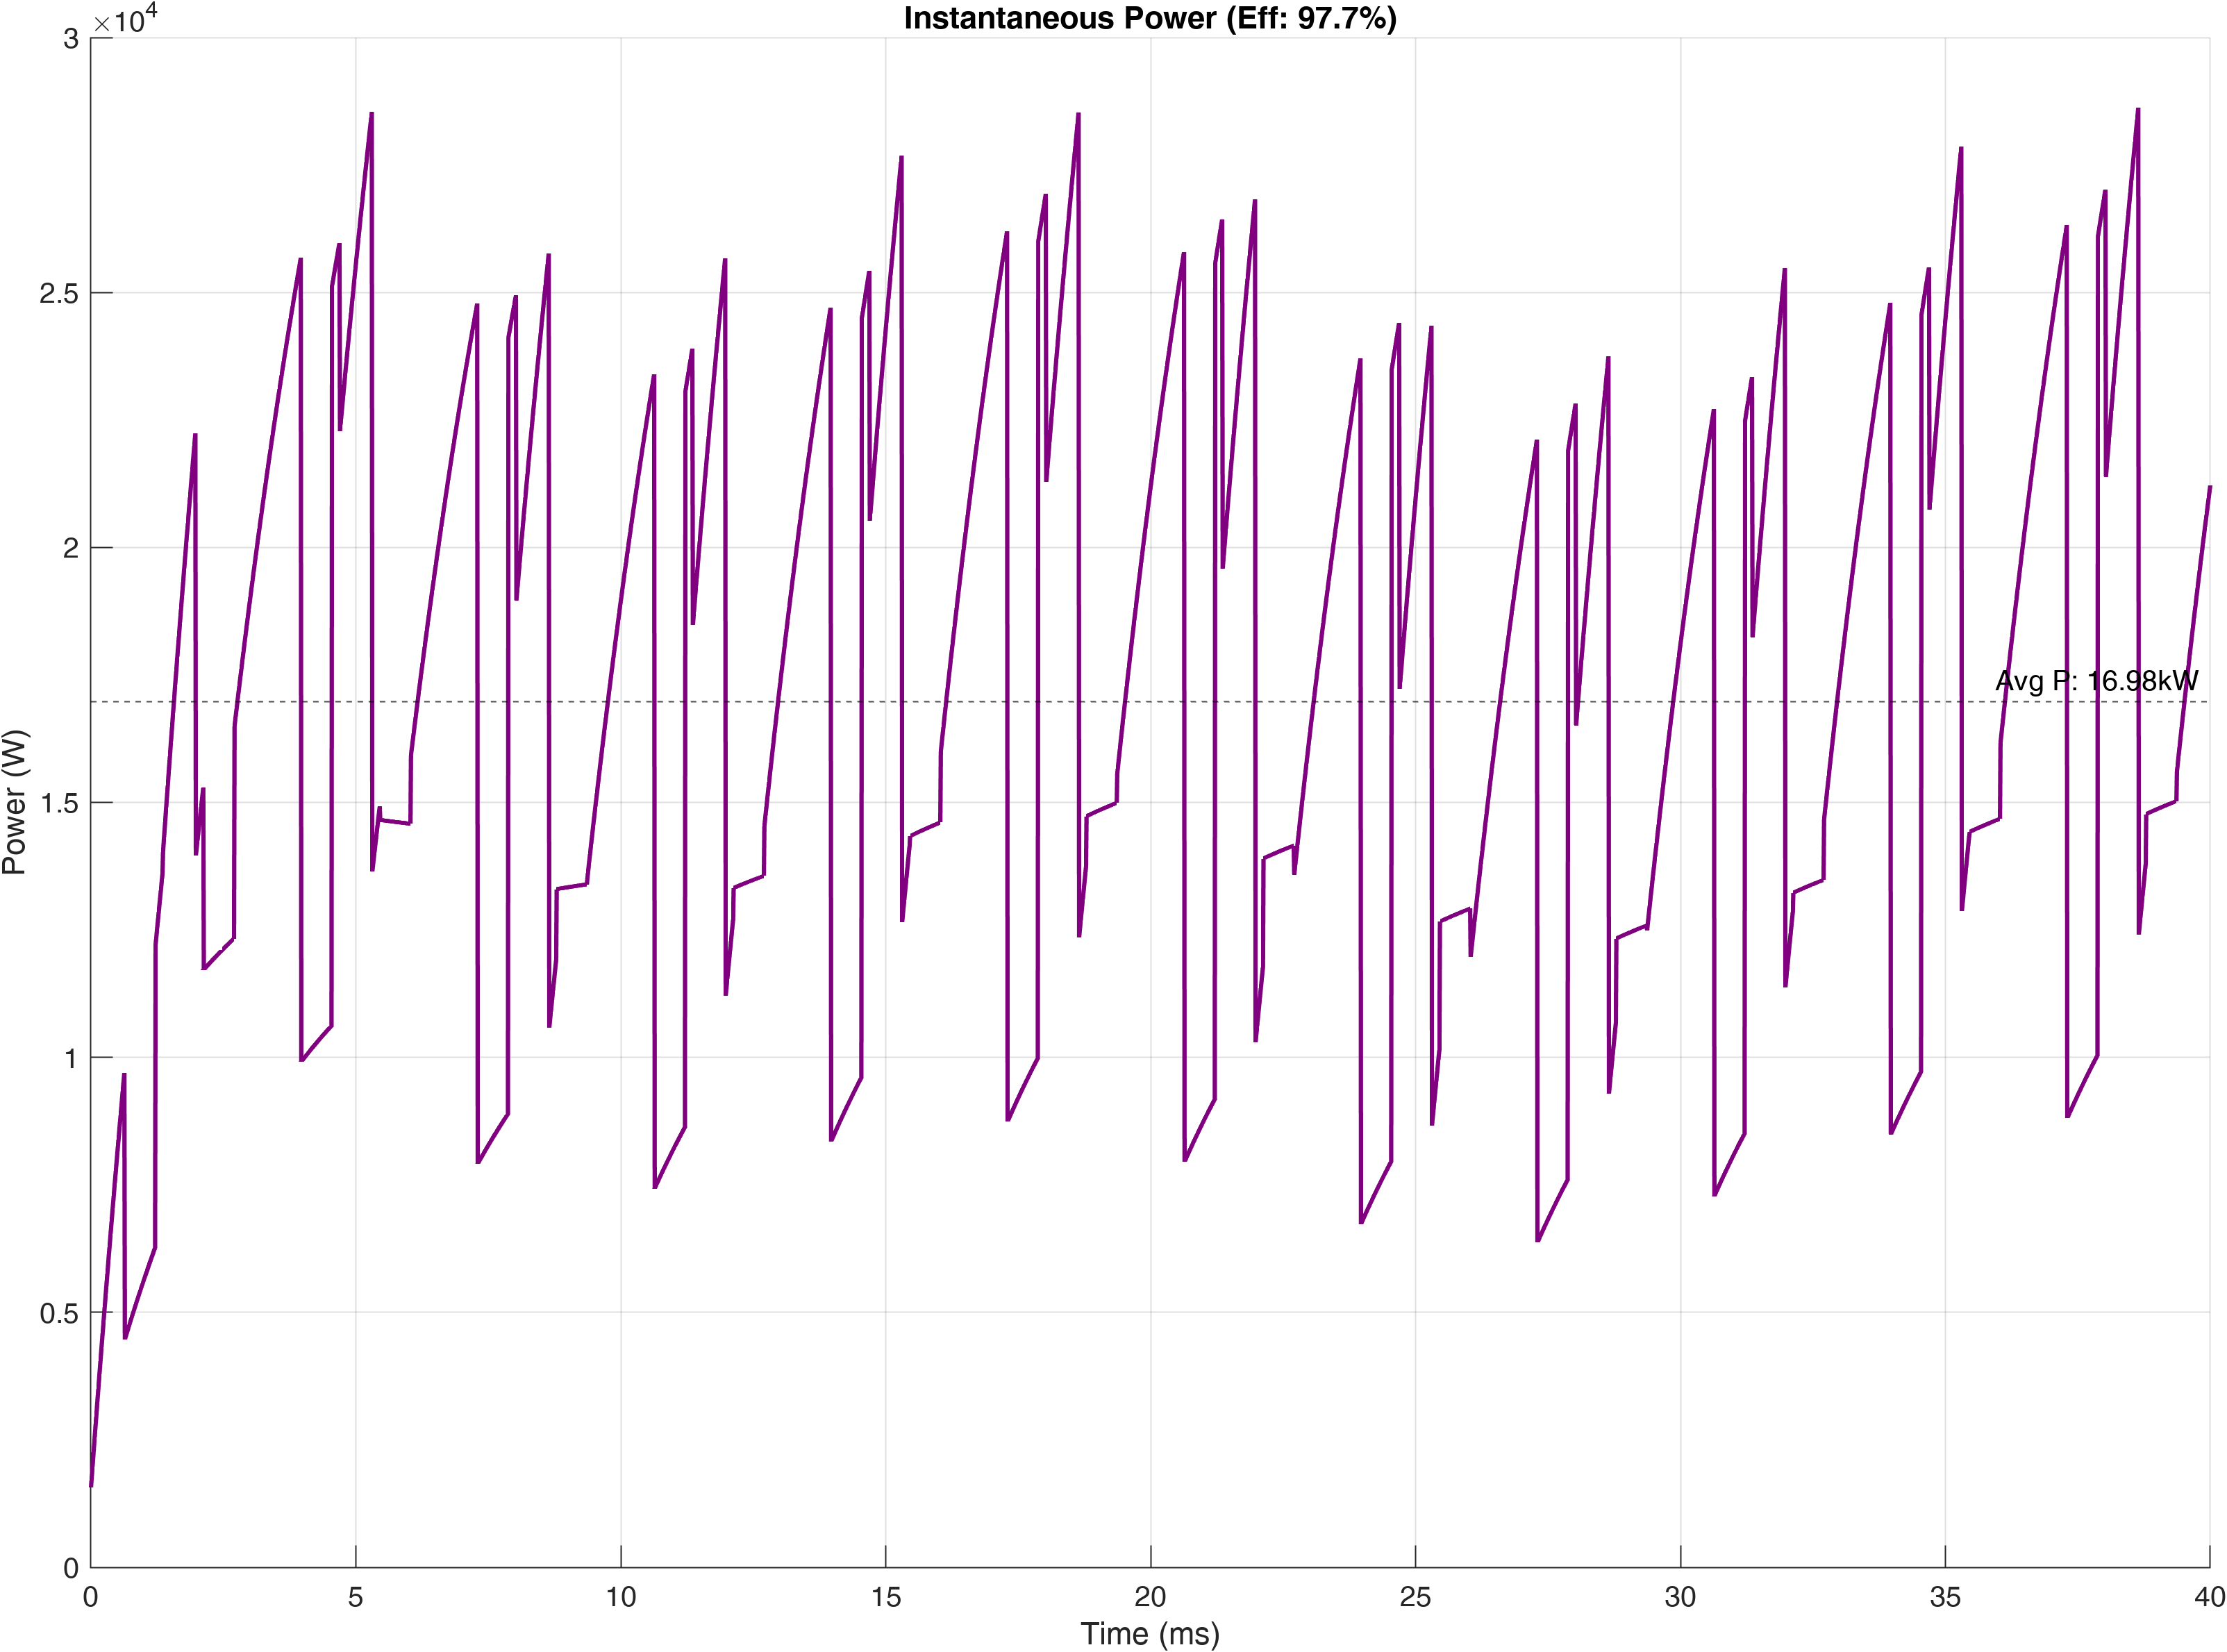
\includegraphics[width=\linewidth]{11_Power_Flow.png}
		\caption{Instantaneous Power Flow Profile}
	\end{figure}
	
	\textbf{Discussion and Analysis:}
	The calculated power factor of $0.67$ precisely matches the theoretical prediction based on the load impedance angle ($\phi = \arctan(X_L/R) = 45^\circ$, resulting in $\cos(45^\circ) \approx 0.707$). The minor deviation is due to the harmonic components in the current. The instantaneous power graph reveals a dominant DC component of $16.98\text{kW}$ superimposed with high-frequency ripples. These ripples are inherent to the switching operation but are significantly reduced compared to 2-level inverters due to the 5-level line voltage synthesis, leading to smoother torque in potential motor drive applications.
	
	\newpage
	\section{Detailed Gate Signal Verification}
	The individual gate signals for Phase A are presented below to verify the specific T-Type switching sequence.
	
	\begin{figure}[H]
		\centering
		% Stacked vertically, full width
		\begin{subfigure}[b]{1.0\linewidth}
			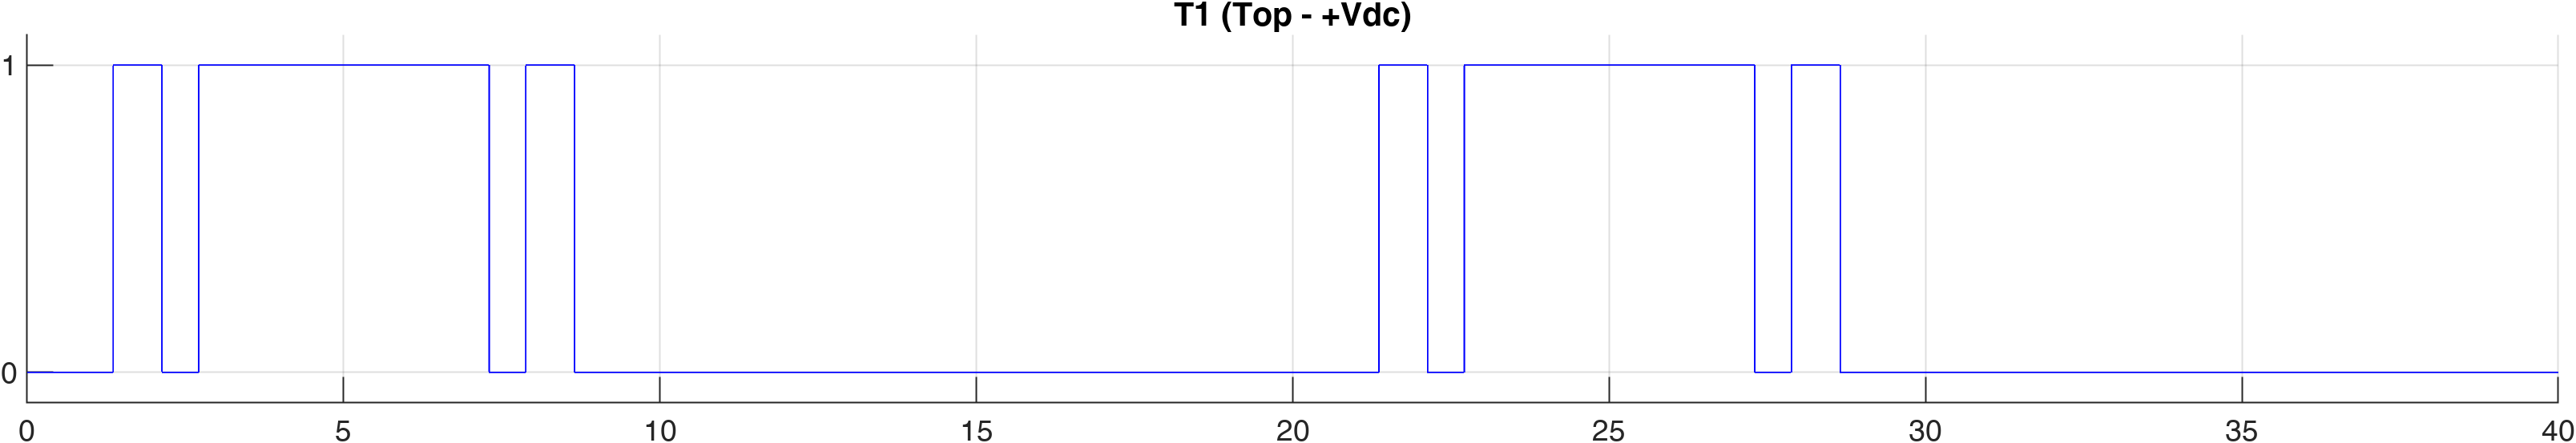
\includegraphics[width=\linewidth]{12_Gate_T1.png}
			\caption{Gate T1 (Positive Rail): Active only during the $+400\text{V}$ peak intervals.}
		\end{subfigure}
		
		\begin{subfigure}[b]{1.0\linewidth}
			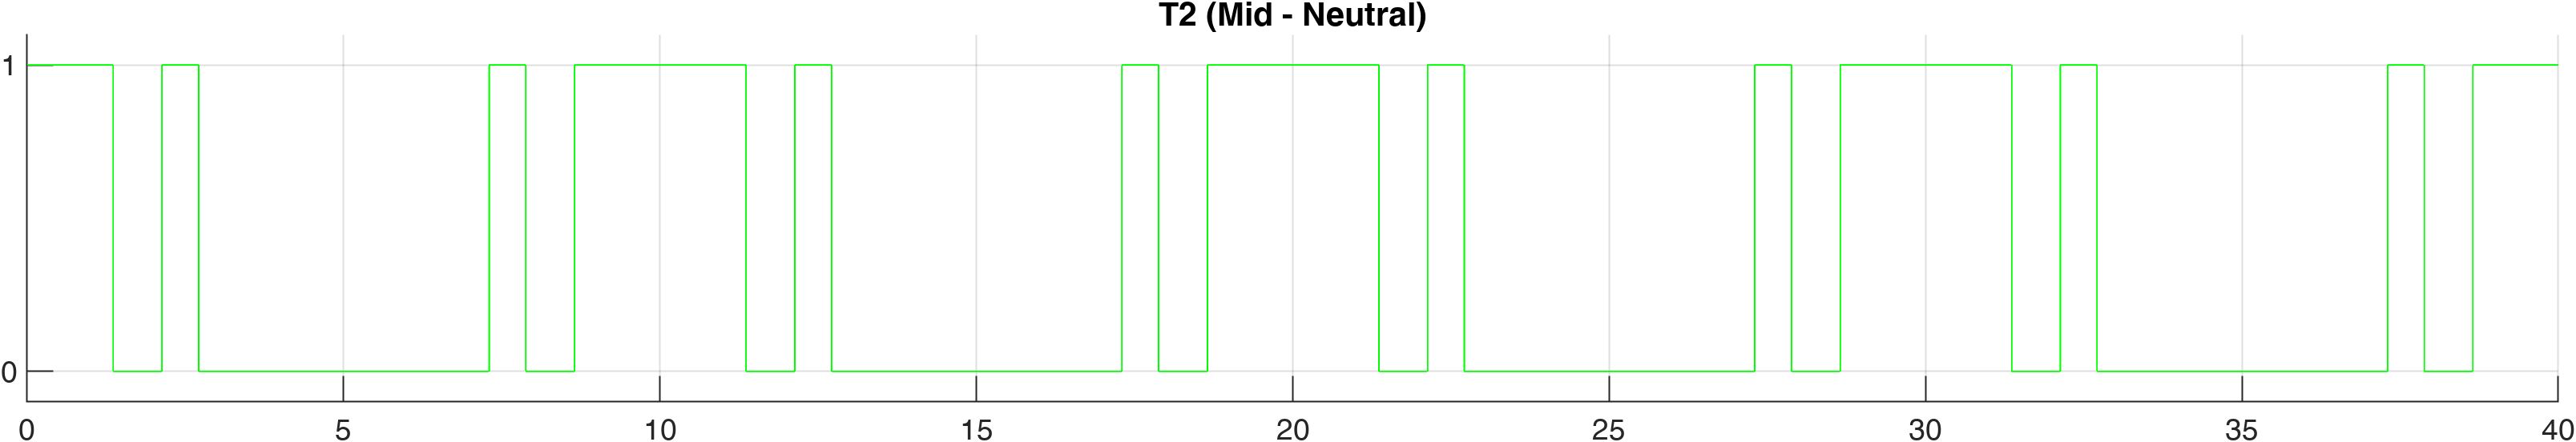
\includegraphics[width=\linewidth]{13_Gate_T2.png}
			\caption{Gate T2 (Neutral Path): Active during zero-voltage clamping intervals.}
		\end{subfigure}
		
		\begin{subfigure}[b]{1.0\linewidth}
			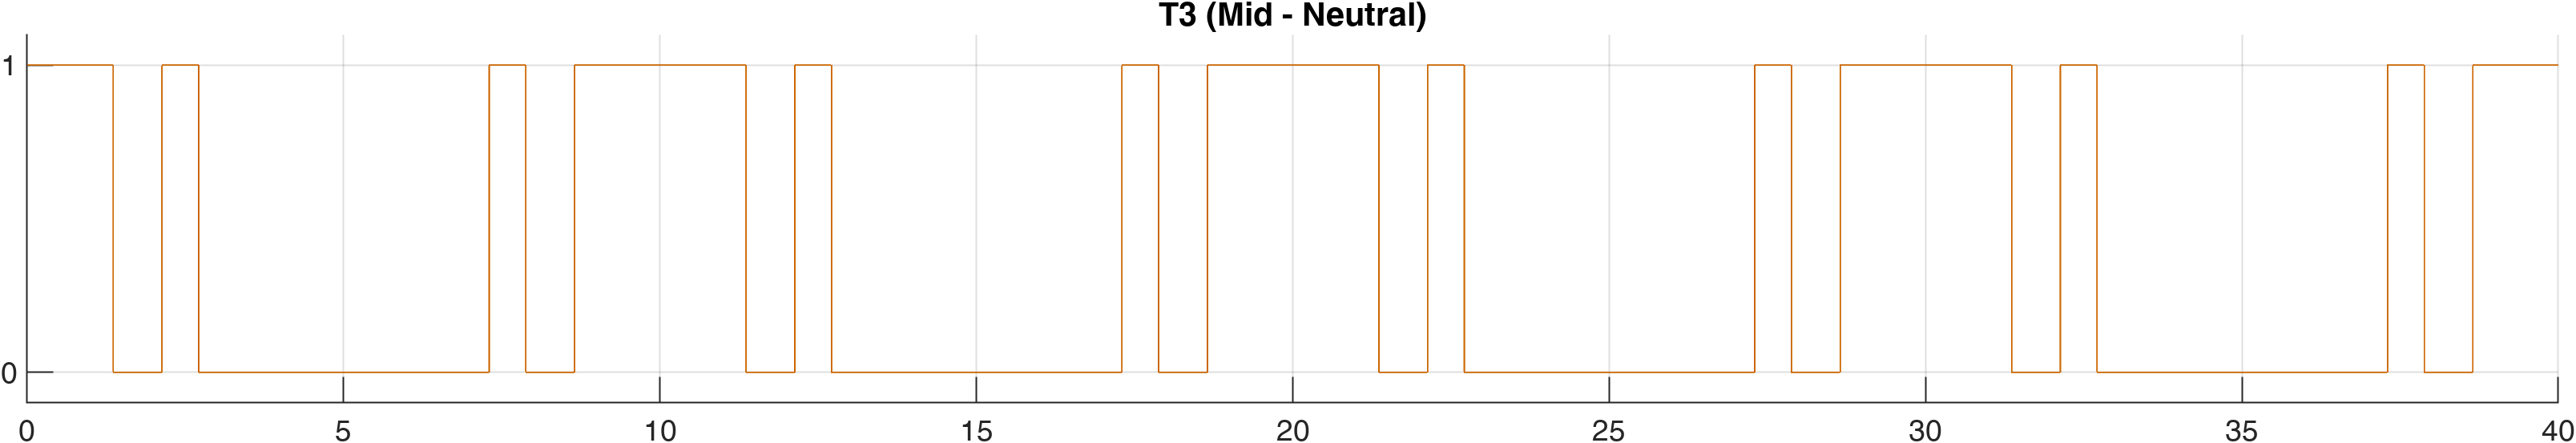
\includegraphics[width=\linewidth]{14_Gate_T3.png}
			\caption{Gate T3 (Neutral Path): Operates in unison with T2 to create the bidirectional neutral path.}
		\end{subfigure}
		
		\begin{subfigure}[b]{1.0\linewidth}
			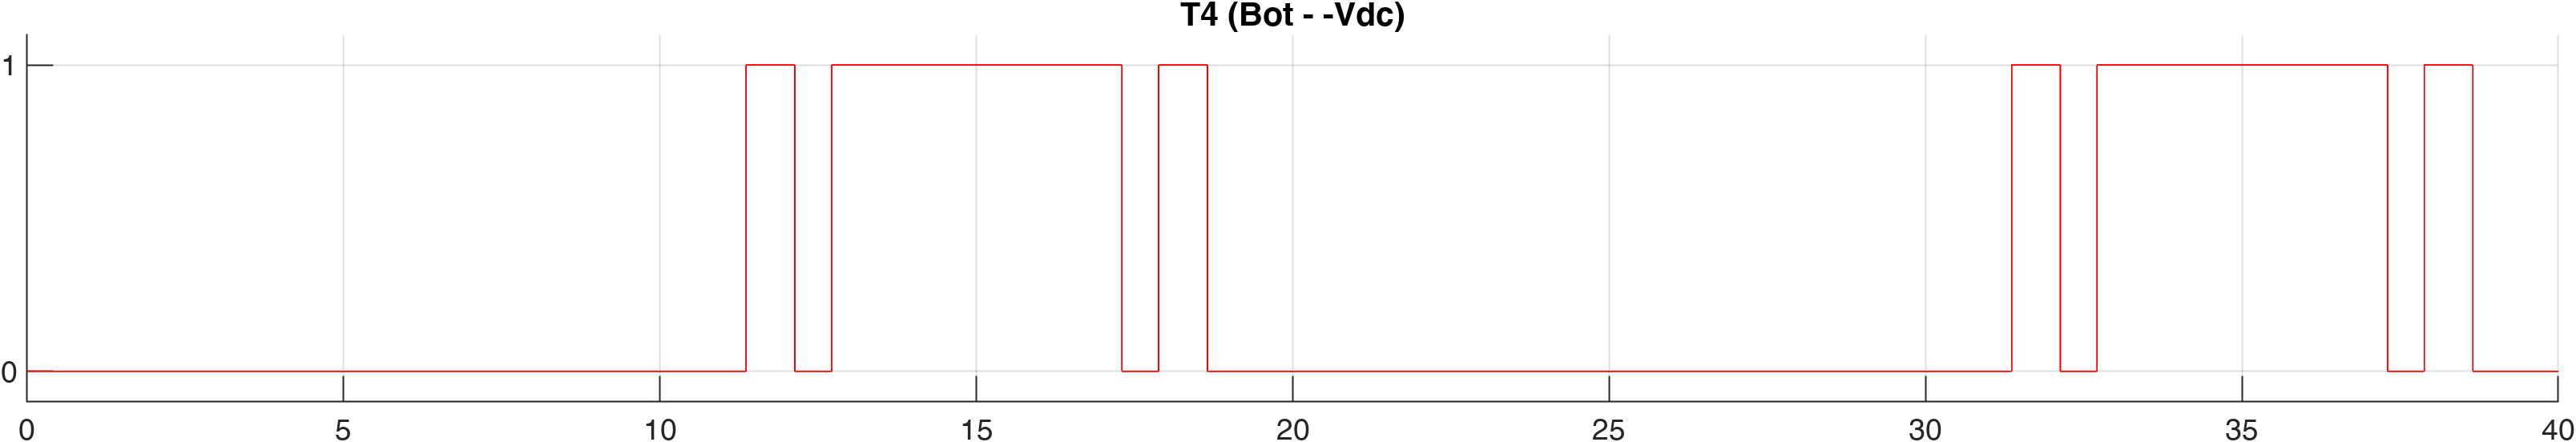
\includegraphics[width=\linewidth]{15_Gate_T4.png}
			\caption{Gate T4 (Negative Rail): Active only during the $-400\text{V}$ negative peak intervals.}
		\end{subfigure}
		\caption{Phase A Gate Drive Signals}
	\end{figure}
	
	\textbf{Switching Sequence Verification:}
	The gate signals confirm the correct T-Type operation mode. Specifically, the "Inner" switches (T2 and T3) are consistently activated during the transition periods between positive and negative half-cycles (the zero states). This validates that the "Fixed" logic correctly identifies the angular intervals $[\alpha_3, \pi-\alpha_3]$ and $[\pi+\alpha_3, 2\pi-\alpha_3]$ where the output must be clamped to the DC midpoint. Furthermore, the absence of overlap between T1 and T4 ensures no DC-link shoot-through faults can occur.
	
	\newpage
	\section{Switching Angle Trajectory Analysis}
	The relationship between the optimal switching angles and the modulation index ($M_a$) is visualized in Figure \ref{fig:traj}.
	
	\begin{figure}[H]
		\centering
		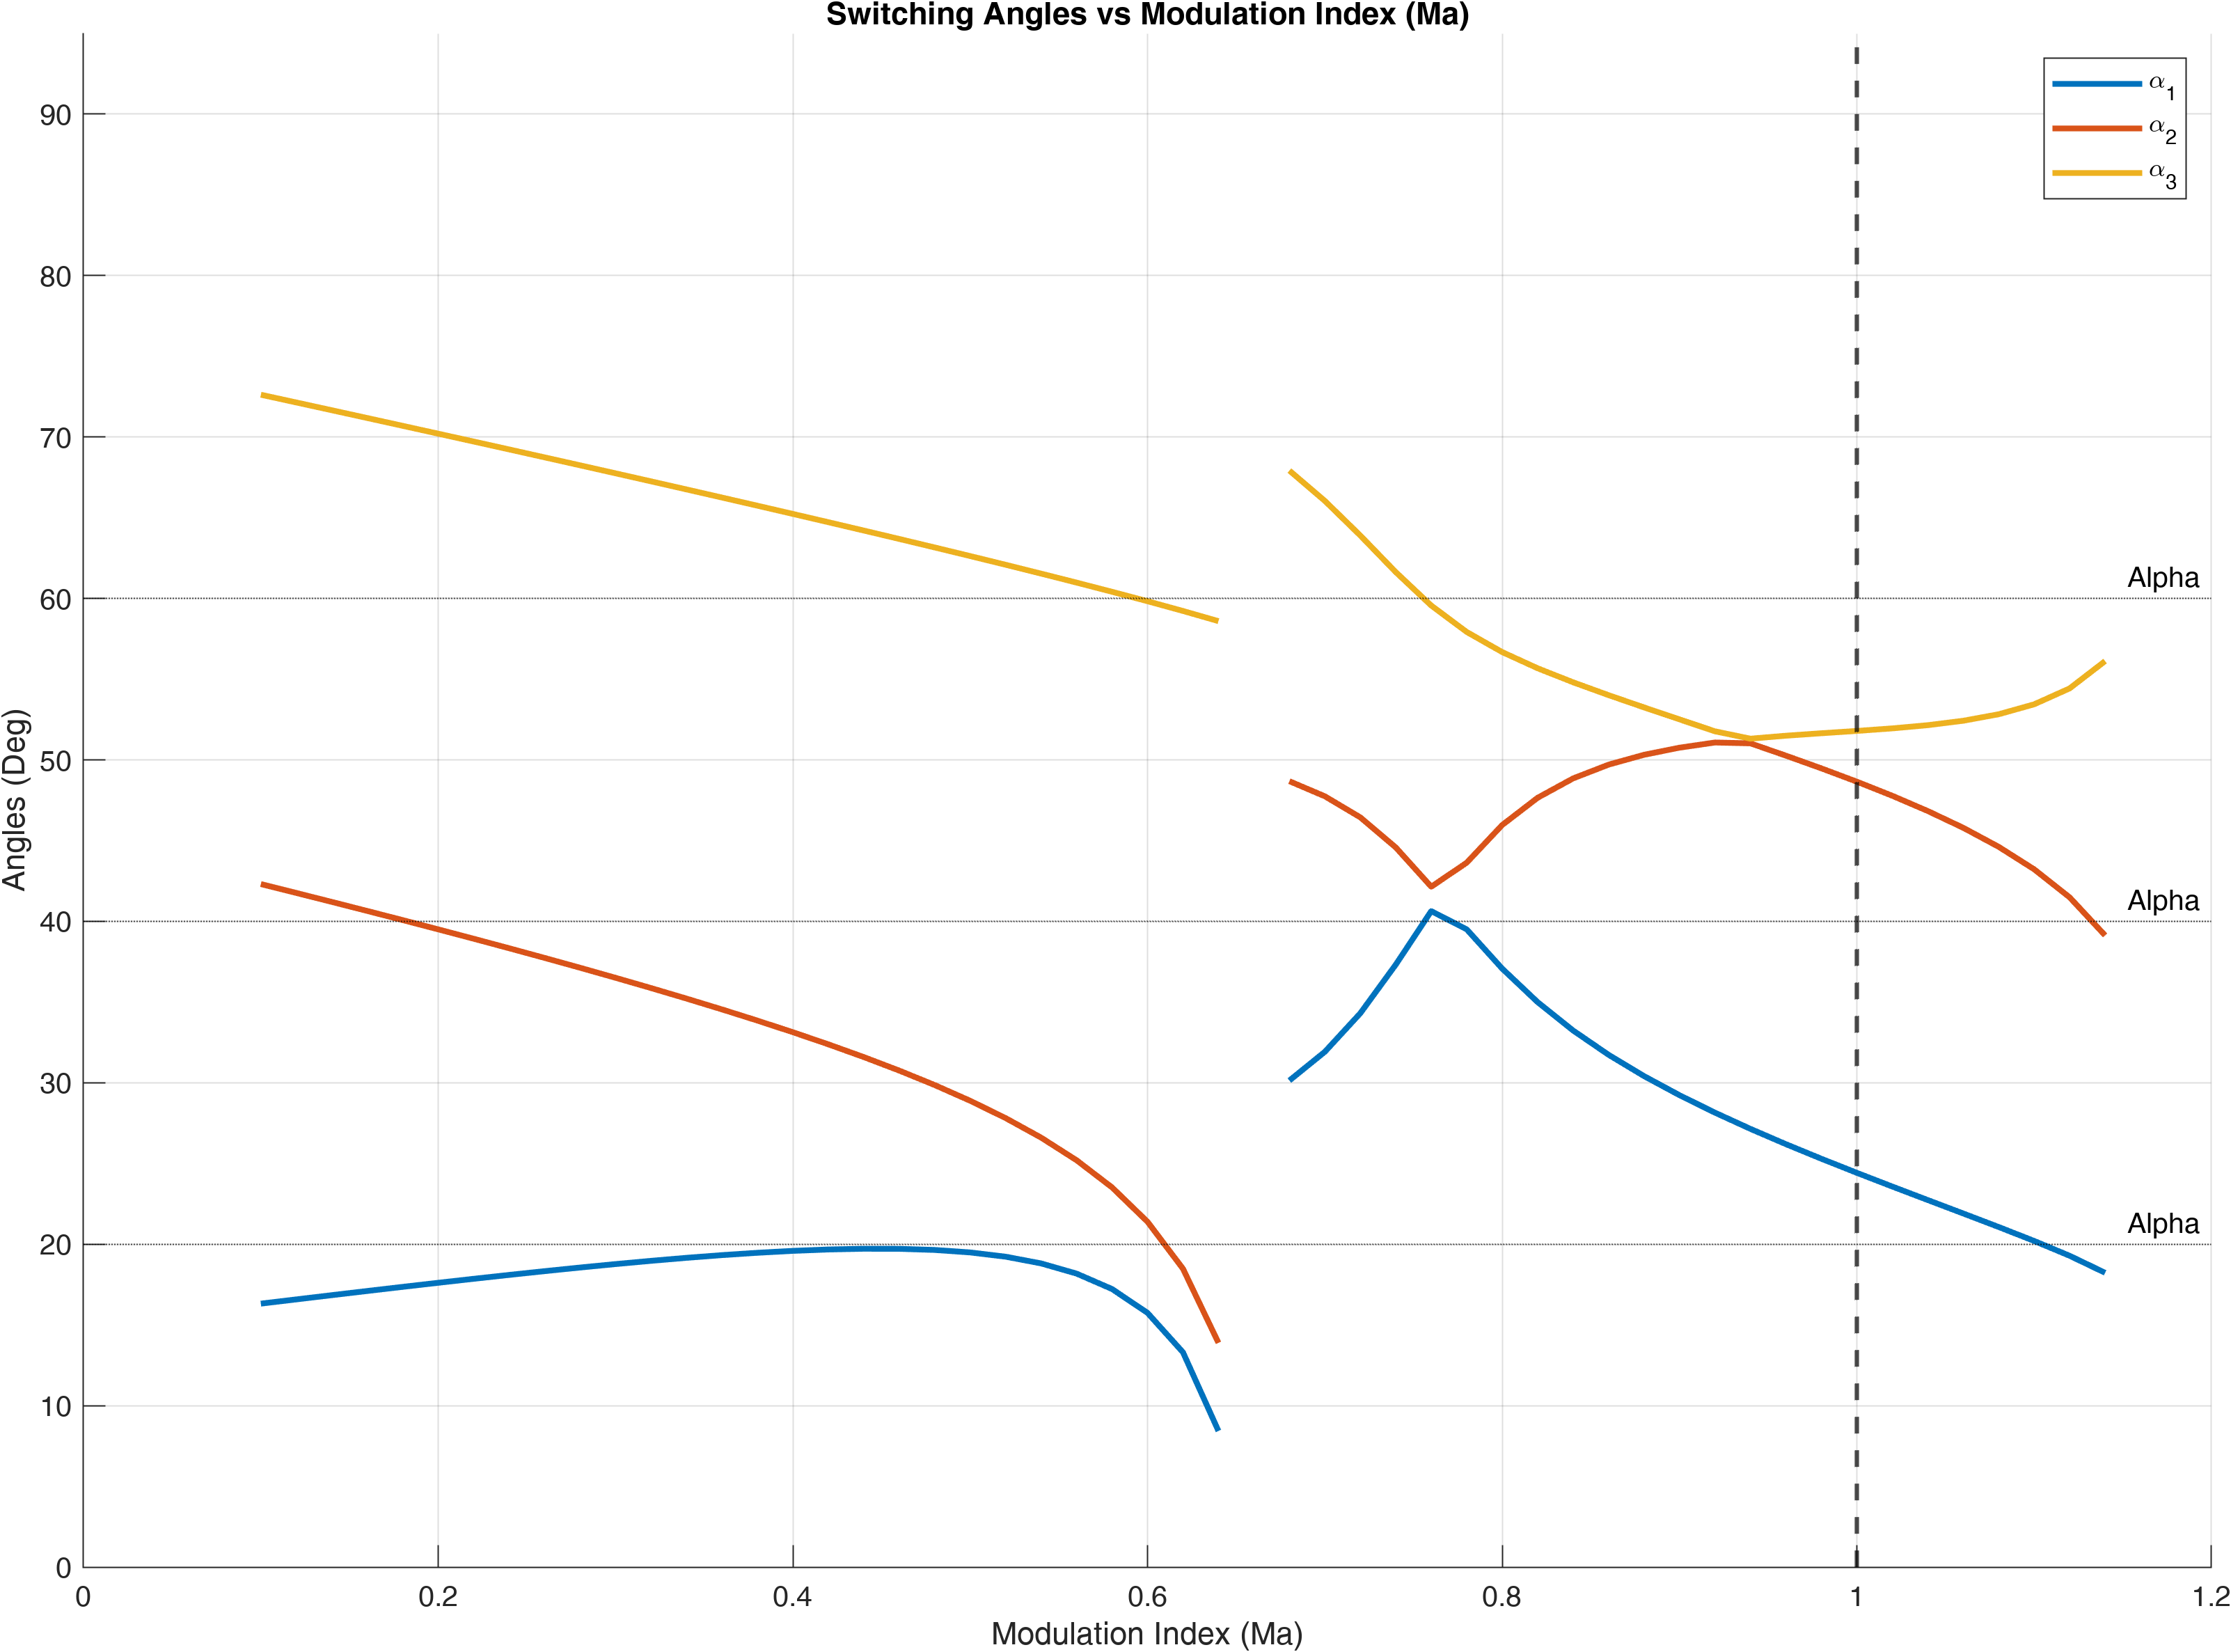
\includegraphics[width=\linewidth]{16_Trajectory_Plot.png}
		\caption{Switching Angle Trajectory vs. Modulation Index}
		\label{fig:traj}
	\end{figure}
	
	\textbf{Interpretation:}
	\begin{itemize}
		\item \textbf{Non-linear Dynamics:} The plot reveals the non-linear dependency of the switching angles on the modulation index. As $M_a$ increases, the pulse widths generally expand to synthesize a higher fundamental voltage.
		\item \textbf{Operating Point:} The vertical dashed line marks the simulation operating point at $M_a = 1.0$. The intersection points yield the specific angles used in this study ($\approx 24.4^\circ, 38.2^\circ, 48.7^\circ$).
		\item \textbf{Solution Stability:} The continuity of the trajectories indicates that valid solutions for eliminating the $5^{th}$ and $7^{th}$ harmonics exist across the entire modulation range, confirming the robustness of the SHE method.
	\end{itemize}
	
	\newpage 
	\section{Conclusion}
	The design and simulation of the three-phase three-level T-Type inverter utilizing Unipolar SHE control yielded successful results. The following conclusions are drawn:
	\begin{itemize}
		\item The computed switching angles precisely generated the required fundamental voltage of $400\text{V}$.
		\item FFT analysis confirmed the complete suppression of the $5^{th}$ and $7^{th}$ harmonic orders.
		\item The implementation of optimized gate logic, specifically the active neutral clamping during zero states, was crucial for waveform stability.
		\item The system achieved a low Current THD of $2.98\%$, demonstrating high power quality suitable for industrial applications.
	\end{itemize}
	
	\newpage
	\appendix
	\section{MATLAB Simulation App Source Code}
	The MATLAB script below is imported directly from the source file \texttt{SHE\_Inverter\_Task\_Final.m}.
	
	\lstinputlisting[caption=SHE\_Inverter\_Task\_Final.m]{SHE_Inverter_Task_Final.m}
	
\end{document}